\documentclass{book}
\usepackage[a4paper,top=2.5cm,bottom=2.5cm,left=2.5cm,right=2.5cm]{geometry}
\usepackage{makeidx}
\usepackage{natbib}
\usepackage{graphicx}
\usepackage{multicol}
\usepackage{float}
\usepackage{listings}
\usepackage{color}
\usepackage{ifthen}
\usepackage[table]{xcolor}
\usepackage{textcomp}
\usepackage{alltt}
\usepackage{ifpdf}
\ifpdf
\usepackage[pdftex,
            pagebackref=true,
            colorlinks=true,
            linkcolor=blue,
            unicode
           ]{hyperref}
\else
\usepackage[ps2pdf,
            pagebackref=true,
            colorlinks=true,
            linkcolor=blue,
            unicode
           ]{hyperref}
\usepackage{pspicture}
\fi
\usepackage[utf8]{inputenc}
\usepackage{mathptmx}
\usepackage[scaled=.90]{helvet}
\usepackage{courier}
\usepackage{sectsty}
\usepackage{amssymb}
\usepackage[titles]{tocloft}
\usepackage{doxygen}
\lstset{language=C++,inputencoding=utf8,basicstyle=\footnotesize,breaklines=true,breakatwhitespace=true,tabsize=4,numbers=left }
\makeindex
\setcounter{tocdepth}{3}
\renewcommand{\footrulewidth}{0.4pt}
\renewcommand{\familydefault}{\sfdefault}
\hfuzz=15pt
\setlength{\emergencystretch}{15pt}
\hbadness=750
\tolerance=750
\begin{document}
\hypersetup{pageanchor=false,citecolor=blue}
\begin{titlepage}
\vspace*{7cm}
\begin{center}
{\Large Linked\-List }\\
\vspace*{1cm}
{\large Generated by Doxygen 1.8.2}\\
\vspace*{0.5cm}
{\small Fri Feb 5 2016 15:14:10}\\
\end{center}
\end{titlepage}
\clearemptydoublepage
\pagenumbering{roman}
\tableofcontents
\clearemptydoublepage
\pagenumbering{arabic}
\hypersetup{pageanchor=true,citecolor=blue}
\chapter{Hierarchical Index}
\section{Class Hierarchy}
This inheritance list is sorted roughly, but not completely, alphabetically\-:\begin{DoxyCompactList}
\item \contentsline{section}{Linked\-List$<$ T $>$}{\pageref{class_linked_list}}{}
\item \contentsline{section}{L\-Ltester$<$ T $>$}{\pageref{class_l_ltester}}{}
\item \contentsline{section}{Node}{\pageref{struct_node}}{}
\item \contentsline{section}{Queue$<$ T $>$}{\pageref{class_queue}}{}
\item \contentsline{section}{Stack$<$ T $>$}{\pageref{class_stack}}{}
\item \contentsline{section}{Stack$<$ int $>$}{\pageref{class_stack}}{}
\begin{DoxyCompactList}
\item \contentsline{section}{Linked\-List\-\_\-\-Arr$<$ T $>$}{\pageref{class_linked_list___arr}}{}
\end{DoxyCompactList}
\end{DoxyCompactList}

\chapter{Class Index}
\section{Class List}
Here are the classes, structs, unions and interfaces with brief descriptions\-:\begin{DoxyCompactList}
\item\contentsline{section}{\hyperlink{class_bucketsort}{Bucketsort} }{\pageref{class_bucketsort}}{}
\item\contentsline{section}{\hyperlink{class_heapsort}{Heapsort} }{\pageref{class_heapsort}}{}
\item\contentsline{section}{\hyperlink{class_insertionsort}{Insertionsort} }{\pageref{class_insertionsort}}{}
\item\contentsline{section}{\hyperlink{classquicksort}{quicksort} }{\pageref{classquicksort}}{}
\item\contentsline{section}{\hyperlink{classrandtime}{randtime} }{\pageref{classrandtime}}{}
\item\contentsline{section}{\hyperlink{class_vector___bucket}{Vector\-\_\-\-Bucket} }{\pageref{class_vector___bucket}}{}
\item\contentsline{section}{\hyperlink{class_vector___heap}{Vector\-\_\-\-Heap} }{\pageref{class_vector___heap}}{}
\item\contentsline{section}{\hyperlink{class_vector___insertion}{Vector\-\_\-\-Insertion} }{\pageref{class_vector___insertion}}{}
\item\contentsline{section}{\hyperlink{class_vector___quick}{Vector\-\_\-\-Quick} }{\pageref{class_vector___quick}}{}
\item\contentsline{section}{\hyperlink{class_vector___rand}{Vector\-\_\-\-Rand} }{\pageref{class_vector___rand}}{}
\end{DoxyCompactList}

\chapter{File Index}
\section{File List}
Here is a list of all files with brief descriptions\-:\begin{DoxyCompactList}
\item\contentsline{section}{//afs/ltu.\-se/students/all/ponste-\/5/\-My Documents/\-Programmering\-\_\-\-Labbar/\-D0041\-D/\-Labb01/\-Linked\-List/\hyperlink{_array__v2_8h}{Array\-\_\-v2.\-h} }{\pageref{_array__v2_8h}}{}
\item\contentsline{section}{//afs/ltu.\-se/students/all/ponste-\/5/\-My Documents/\-Programmering\-\_\-\-Labbar/\-D0041\-D/\-Labb01/\-Linked\-List/\hyperlink{_linked_list_8cpp}{Linked\-List.\-cpp} }{\pageref{_linked_list_8cpp}}{}
\item\contentsline{section}{//afs/ltu.\-se/students/all/ponste-\/5/\-My Documents/\-Programmering\-\_\-\-Labbar/\-D0041\-D/\-Labb01/\-Linked\-List/\hyperlink{_linked_list_8h}{Linked\-List.\-h} }{\pageref{_linked_list_8h}}{}
\item\contentsline{section}{//afs/ltu.\-se/students/all/ponste-\/5/\-My Documents/\-Programmering\-\_\-\-Labbar/\-D0041\-D/\-Labb01/\-Linked\-List/\hyperlink{_list___array_8cpp}{List\-\_\-\-Array.\-cpp} }{\pageref{_list___array_8cpp}}{}
\item\contentsline{section}{//afs/ltu.\-se/students/all/ponste-\/5/\-My Documents/\-Programmering\-\_\-\-Labbar/\-D0041\-D/\-Labb01/\-Linked\-List/\hyperlink{_list___array_8h}{List\-\_\-\-Array.\-h} }{\pageref{_list___array_8h}}{}
\item\contentsline{section}{//afs/ltu.\-se/students/all/ponste-\/5/\-My Documents/\-Programmering\-\_\-\-Labbar/\-D0041\-D/\-Labb01/\-Linked\-List/\hyperlink{listchecks_8h}{listchecks.\-h} }{\pageref{listchecks_8h}}{}
\item\contentsline{section}{//afs/ltu.\-se/students/all/ponste-\/5/\-My Documents/\-Programmering\-\_\-\-Labbar/\-D0041\-D/\-Labb01/\-Linked\-List/\hyperlink{_main_07_08_8cpp}{Main().\-cpp} }{\pageref{_main_07_08_8cpp}}{}
\item\contentsline{section}{//afs/ltu.\-se/students/all/ponste-\/5/\-My Documents/\-Programmering\-\_\-\-Labbar/\-D0041\-D/\-Labb01/\-Linked\-List/\hyperlink{_main_8cpp}{Main.\-cpp} }{\pageref{_main_8cpp}}{}
\item\contentsline{section}{//afs/ltu.\-se/students/all/ponste-\/5/\-My Documents/\-Programmering\-\_\-\-Labbar/\-D0041\-D/\-Labb01/\-Linked\-List/\hyperlink{_queue_8h}{Queue.\-h} }{\pageref{_queue_8h}}{}
\item\contentsline{section}{//afs/ltu.\-se/students/all/ponste-\/5/\-My Documents/\-Programmering\-\_\-\-Labbar/\-D0041\-D/\-Labb01/\-Linked\-List/\hyperlink{_stack_8h}{Stack.\-h} }{\pageref{_stack_8h}}{}
\item\contentsline{section}{//afs/ltu.\-se/students/all/ponste-\/5/\-My Documents/\-Programmering\-\_\-\-Labbar/\-D0041\-D/\-Labb01/\-Linked\-List/\hyperlink{_stack__v2_8h}{Stack\-\_\-v2.\-h} }{\pageref{_stack__v2_8h}}{}
\item\contentsline{section}{//afs/ltu.\-se/students/all/ponste-\/5/\-My Documents/\-Programmering\-\_\-\-Labbar/\-D0041\-D/\-Labb01/\-Linked\-List/\hyperlink{_unit__test_8cpp}{Unit\-\_\-test.\-cpp} }{\pageref{_unit__test_8cpp}}{}
\item\contentsline{section}{//afs/ltu.\-se/students/all/ponste-\/5/\-My Documents/\-Programmering\-\_\-\-Labbar/\-D0041\-D/\-Labb01/\-Linked\-List/\hyperlink{_unit__test_8h}{Unit\-\_\-test.\-h} }{\pageref{_unit__test_8h}}{}
\end{DoxyCompactList}

\chapter{Class Documentation}
\hypertarget{class_linked_list}{\section{Linked\-List$<$ T $>$ Class Template Reference}
\label{class_linked_list}\index{Linked\-List$<$ T $>$@{Linked\-List$<$ T $>$}}
}


{\ttfamily \#include $<$Linked\-List.\-h$>$}

\subsection*{Public Member Functions}
\begin{DoxyCompactItemize}
\item 
\hyperlink{class_linked_list_a3c20fcfec867e867f541061a09fc640c}{Linked\-List} ()
\item 
\hyperlink{class_linked_list_a7c37609df3b83bc4eb0281b852f93fd7}{$\sim$\-Linked\-List} ()
\item 
bool \hyperlink{class_linked_list_a66623a06d807357884006e8724c82297}{is\-Off} ()
\item 
int \hyperlink{class_linked_list_a5d442d070c04f5a223ba3963a092b916}{item} ()
\item 
void \hyperlink{class_linked_list_a46632fdbf5a64821dbe642070416b7c6}{start} ()
\item 
void \hyperlink{class_linked_list_a5c00242d2105ab8057af3efa68c18af4}{forth} ()
\item 
void \hyperlink{class_linked_list_a467c23980e0c463c12a3a820743b180b}{insert\-Before} (int num)
\item 
void \hyperlink{class_linked_list_ae28327cccd9acd61c33a6b51631ffdee}{remove\-At} ()
\item 
int \hyperlink{class_linked_list_a7eba1203d539345805a669f2ca23cf66}{Get\-\_\-\-Size} ()
\item 
\hyperlink{class_linked_list_a7bf2d4b9ac8f9bb493e4e1237adb981a}{Linked\-List} (int size)
\item 
\hyperlink{class_linked_list_a7c37609df3b83bc4eb0281b852f93fd7}{$\sim$\-Linked\-List} ()
\item 
bool \hyperlink{class_linked_list_a66623a06d807357884006e8724c82297}{is\-Off} ()
\item 
T \hyperlink{class_linked_list_a5d442d070c04f5a223ba3963a092b916}{item} ()
\item 
void \hyperlink{class_linked_list_a46632fdbf5a64821dbe642070416b7c6}{start} ()
\item 
void \hyperlink{class_linked_list_a5c00242d2105ab8057af3efa68c18af4}{forth} ()
\item 
void \hyperlink{class_linked_list_ad88b2169453b763c78ba739551857db4}{insert\-Before} (T data)
\item 
void \hyperlink{class_linked_list_ae28327cccd9acd61c33a6b51631ffdee}{remove\-At} ()
\item 
void \hyperlink{class_linked_list_a3a83eb87f262980e4681e4c94ee05136}{whole} ()
\end{DoxyCompactItemize}
\subsection*{Protected Attributes}
\begin{DoxyCompactItemize}
\item 
\hyperlink{struct_node}{Node} $\ast$ \hyperlink{class_linked_list_a2d1f848e19caa3f180b7fa6938125bba}{head}
\item 
\hyperlink{struct_node}{Node} $\ast$ \hyperlink{class_linked_list_ac31fae6ecb440b8d069790e5294f82fe}{current}
\item 
\hyperlink{struct_node}{Node} $\ast$ \hyperlink{class_linked_list_a3489a27822d31002e3ffeea44b402296}{previous}
\item 
int \hyperlink{class_linked_list_affff5ce490bbe41e4d1bcb21b846891c}{list\-\_\-size}
\item 
int \hyperlink{class_linked_list_a2e6a6b5a560b362c8f03cca2183c2710}{head}
\item 
int \hyperlink{class_linked_list_ae6821bb450a08c7e918e477b747667c1}{iteratos\-Pos}
\item 
int \hyperlink{class_linked_list_ad8fb5d6184b9d23087bd4916722ee3ae}{previous}
\end{DoxyCompactItemize}


\subsection{Constructor \& Destructor Documentation}
\hypertarget{class_linked_list_a3c20fcfec867e867f541061a09fc640c}{\index{Linked\-List@{Linked\-List}!Linked\-List@{Linked\-List}}
\index{Linked\-List@{Linked\-List}!LinkedList@{Linked\-List}}
\subsubsection[{Linked\-List}]{\setlength{\rightskip}{0pt plus 5cm}template$<$class T $>$ {\bf Linked\-List}$<$ T $>$\-::{\bf Linked\-List} (
\begin{DoxyParamCaption}
{}
\end{DoxyParamCaption}
)}}\label{class_linked_list_a3c20fcfec867e867f541061a09fc640c}
\hypertarget{class_linked_list_a7c37609df3b83bc4eb0281b852f93fd7}{\index{Linked\-List@{Linked\-List}!$\sim$\-Linked\-List@{$\sim$\-Linked\-List}}
\index{$\sim$\-Linked\-List@{$\sim$\-Linked\-List}!LinkedList@{Linked\-List}}
\subsubsection[{$\sim$\-Linked\-List}]{\setlength{\rightskip}{0pt plus 5cm}template$<$class T $>$ {\bf Linked\-List}$<$ T $>$\-::$\sim${\bf Linked\-List} (
\begin{DoxyParamCaption}
{}
\end{DoxyParamCaption}
)}}\label{class_linked_list_a7c37609df3b83bc4eb0281b852f93fd7}
\hypertarget{class_linked_list_a7bf2d4b9ac8f9bb493e4e1237adb981a}{\index{Linked\-List@{Linked\-List}!Linked\-List@{Linked\-List}}
\index{Linked\-List@{Linked\-List}!LinkedList@{Linked\-List}}
\subsubsection[{Linked\-List}]{\setlength{\rightskip}{0pt plus 5cm}template$<$class T $>$ {\bf Linked\-List}$<$ T $>$\-::{\bf Linked\-List} (
\begin{DoxyParamCaption}
\item[{int}]{size}
\end{DoxyParamCaption}
)}}\label{class_linked_list_a7bf2d4b9ac8f9bb493e4e1237adb981a}
\hypertarget{class_linked_list_a7c37609df3b83bc4eb0281b852f93fd7}{\index{Linked\-List@{Linked\-List}!$\sim$\-Linked\-List@{$\sim$\-Linked\-List}}
\index{$\sim$\-Linked\-List@{$\sim$\-Linked\-List}!LinkedList@{Linked\-List}}
\subsubsection[{$\sim$\-Linked\-List}]{\setlength{\rightskip}{0pt plus 5cm}template$<$class T $>$ {\bf Linked\-List}$<$ T $>$\-::$\sim${\bf Linked\-List} (
\begin{DoxyParamCaption}
{}
\end{DoxyParamCaption}
)}}\label{class_linked_list_a7c37609df3b83bc4eb0281b852f93fd7}


\subsection{Member Function Documentation}
\hypertarget{class_linked_list_a5c00242d2105ab8057af3efa68c18af4}{\index{Linked\-List@{Linked\-List}!forth@{forth}}
\index{forth@{forth}!LinkedList@{Linked\-List}}
\subsubsection[{forth}]{\setlength{\rightskip}{0pt plus 5cm}template$<$class T $>$ void {\bf Linked\-List}$<$ T $>$\-::forth (
\begin{DoxyParamCaption}
{}
\end{DoxyParamCaption}
)}}\label{class_linked_list_a5c00242d2105ab8057af3efa68c18af4}
\hypertarget{class_linked_list_a5c00242d2105ab8057af3efa68c18af4}{\index{Linked\-List@{Linked\-List}!forth@{forth}}
\index{forth@{forth}!LinkedList@{Linked\-List}}
\subsubsection[{forth}]{\setlength{\rightskip}{0pt plus 5cm}template$<$class T $>$ void {\bf Linked\-List}$<$ T $>$\-::forth (
\begin{DoxyParamCaption}
{}
\end{DoxyParamCaption}
)}}\label{class_linked_list_a5c00242d2105ab8057af3efa68c18af4}
$\ast$\-Points current and previous a to Nodes next \hypertarget{class_linked_list_a7eba1203d539345805a669f2ca23cf66}{\index{Linked\-List@{Linked\-List}!Get\-\_\-\-Size@{Get\-\_\-\-Size}}
\index{Get\-\_\-\-Size@{Get\-\_\-\-Size}!LinkedList@{Linked\-List}}
\subsubsection[{Get\-\_\-\-Size}]{\setlength{\rightskip}{0pt plus 5cm}template$<$class T $>$ int {\bf Linked\-List}$<$ T $>$\-::Get\-\_\-\-Size (
\begin{DoxyParamCaption}
{}
\end{DoxyParamCaption}
)}}\label{class_linked_list_a7eba1203d539345805a669f2ca23cf66}
$\ast$\-Method that is used in unit tester \hypertarget{class_linked_list_ad88b2169453b763c78ba739551857db4}{\index{Linked\-List@{Linked\-List}!insert\-Before@{insert\-Before}}
\index{insert\-Before@{insert\-Before}!LinkedList@{Linked\-List}}
\subsubsection[{insert\-Before}]{\setlength{\rightskip}{0pt plus 5cm}template$<$class T $>$ void {\bf Linked\-List}$<$ T $>$\-::insert\-Before (
\begin{DoxyParamCaption}
\item[{T}]{data}
\end{DoxyParamCaption}
)}}\label{class_linked_list_ad88b2169453b763c78ba739551857db4}
\hypertarget{class_linked_list_a467c23980e0c463c12a3a820743b180b}{\index{Linked\-List@{Linked\-List}!insert\-Before@{insert\-Before}}
\index{insert\-Before@{insert\-Before}!LinkedList@{Linked\-List}}
\subsubsection[{insert\-Before}]{\setlength{\rightskip}{0pt plus 5cm}template$<$class T $>$ void {\bf Linked\-List}$<$ T $>$\-::insert\-Before (
\begin{DoxyParamCaption}
\item[{int}]{num}
\end{DoxyParamCaption}
)}}\label{class_linked_list_a467c23980e0c463c12a3a820743b180b}
$\ast$\-Inserts a new \hyperlink{struct_node}{Node} between current and previous $\ast$\-Points the new Nodes next to current $\ast$\-Points previous next to the new \hyperlink{struct_node}{Node} $\ast$\-Points previous to the new \hyperlink{struct_node}{Node} \hypertarget{class_linked_list_a66623a06d807357884006e8724c82297}{\index{Linked\-List@{Linked\-List}!is\-Off@{is\-Off}}
\index{is\-Off@{is\-Off}!LinkedList@{Linked\-List}}
\subsubsection[{is\-Off}]{\setlength{\rightskip}{0pt plus 5cm}template$<$class T $>$ bool {\bf Linked\-List}$<$ T $>$\-::is\-Off (
\begin{DoxyParamCaption}
{}
\end{DoxyParamCaption}
)}}\label{class_linked_list_a66623a06d807357884006e8724c82297}
\hypertarget{class_linked_list_a66623a06d807357884006e8724c82297}{\index{Linked\-List@{Linked\-List}!is\-Off@{is\-Off}}
\index{is\-Off@{is\-Off}!LinkedList@{Linked\-List}}
\subsubsection[{is\-Off}]{\setlength{\rightskip}{0pt plus 5cm}template$<$class T $>$ bool {\bf Linked\-List}$<$ T $>$\-::is\-Off (
\begin{DoxyParamCaption}
{}
\end{DoxyParamCaption}
)}}\label{class_linked_list_a66623a06d807357884006e8724c82297}
$\ast$\-Checks if current == nullptr  true/false \hypertarget{class_linked_list_a5d442d070c04f5a223ba3963a092b916}{\index{Linked\-List@{Linked\-List}!item@{item}}
\index{item@{item}!LinkedList@{Linked\-List}}
\subsubsection[{item}]{\setlength{\rightskip}{0pt plus 5cm}template$<$class T $>$ T {\bf Linked\-List}$<$ T $>$\-::item (
\begin{DoxyParamCaption}
{}
\end{DoxyParamCaption}
)}}\label{class_linked_list_a5d442d070c04f5a223ba3963a092b916}
\hypertarget{class_linked_list_a5d442d070c04f5a223ba3963a092b916}{\index{Linked\-List@{Linked\-List}!item@{item}}
\index{item@{item}!LinkedList@{Linked\-List}}
\subsubsection[{item}]{\setlength{\rightskip}{0pt plus 5cm}template$<$class T $>$ T {\bf Linked\-List}$<$ T $>$\-::item (
\begin{DoxyParamCaption}
{}
\end{DoxyParamCaption}
)}}\label{class_linked_list_a5d442d070c04f5a223ba3963a092b916}
$\ast$\-Checks if\-Off()  the value of the \hyperlink{struct_node}{Node} that current is pointing to \hypertarget{class_linked_list_ae28327cccd9acd61c33a6b51631ffdee}{\index{Linked\-List@{Linked\-List}!remove\-At@{remove\-At}}
\index{remove\-At@{remove\-At}!LinkedList@{Linked\-List}}
\subsubsection[{remove\-At}]{\setlength{\rightskip}{0pt plus 5cm}template$<$class T $>$ void {\bf Linked\-List}$<$ T $>$\-::remove\-At (
\begin{DoxyParamCaption}
{}
\end{DoxyParamCaption}
)}}\label{class_linked_list_ae28327cccd9acd61c33a6b51631ffdee}
\hypertarget{class_linked_list_ae28327cccd9acd61c33a6b51631ffdee}{\index{Linked\-List@{Linked\-List}!remove\-At@{remove\-At}}
\index{remove\-At@{remove\-At}!LinkedList@{Linked\-List}}
\subsubsection[{remove\-At}]{\setlength{\rightskip}{0pt plus 5cm}template$<$class T $>$ void {\bf Linked\-List}$<$ T $>$\-::remove\-At (
\begin{DoxyParamCaption}
{}
\end{DoxyParamCaption}
)}}\label{class_linked_list_ae28327cccd9acd61c33a6b51631ffdee}
$\ast$\-Calls \hyperlink{class_linked_list_a66623a06d807357884006e8724c82297}{is\-Off()} and goes forth is false $\ast$\-Removes the \hyperlink{struct_node}{Node} that current is pointing to and repoints current to its next $\ast$\-Points previous next to \char`\"{}new\char`\"{} current \hypertarget{class_linked_list_a46632fdbf5a64821dbe642070416b7c6}{\index{Linked\-List@{Linked\-List}!start@{start}}
\index{start@{start}!LinkedList@{Linked\-List}}
\subsubsection[{start}]{\setlength{\rightskip}{0pt plus 5cm}template$<$class T $>$ void {\bf Linked\-List}$<$ T $>$\-::start (
\begin{DoxyParamCaption}
{}
\end{DoxyParamCaption}
)}}\label{class_linked_list_a46632fdbf5a64821dbe642070416b7c6}
\hypertarget{class_linked_list_a46632fdbf5a64821dbe642070416b7c6}{\index{Linked\-List@{Linked\-List}!start@{start}}
\index{start@{start}!LinkedList@{Linked\-List}}
\subsubsection[{start}]{\setlength{\rightskip}{0pt plus 5cm}template$<$class T $>$ void {\bf Linked\-List}$<$ T $>$\-::start (
\begin{DoxyParamCaption}
{}
\end{DoxyParamCaption}
)}}\label{class_linked_list_a46632fdbf5a64821dbe642070416b7c6}
$\ast$\-Points current to heads Nodes next $\ast$\-Points previous to the same \hyperlink{struct_node}{Node} as head \hypertarget{class_linked_list_a3a83eb87f262980e4681e4c94ee05136}{\index{Linked\-List@{Linked\-List}!whole@{whole}}
\index{whole@{whole}!LinkedList@{Linked\-List}}
\subsubsection[{whole}]{\setlength{\rightskip}{0pt plus 5cm}template$<$class T $>$ void {\bf Linked\-List}$<$ T $>$\-::whole (
\begin{DoxyParamCaption}
{}
\end{DoxyParamCaption}
)}}\label{class_linked_list_a3a83eb87f262980e4681e4c94ee05136}


\subsection{Member Data Documentation}
\hypertarget{class_linked_list_ac31fae6ecb440b8d069790e5294f82fe}{\index{Linked\-List@{Linked\-List}!current@{current}}
\index{current@{current}!LinkedList@{Linked\-List}}
\subsubsection[{current}]{\setlength{\rightskip}{0pt plus 5cm}template$<$class T $>$ {\bf Node}$\ast$ {\bf Linked\-List}$<$ T $>$\-::current\hspace{0.3cm}{\ttfamily [protected]}}}\label{class_linked_list_ac31fae6ecb440b8d069790e5294f82fe}
\hypertarget{class_linked_list_a2e6a6b5a560b362c8f03cca2183c2710}{\index{Linked\-List@{Linked\-List}!head@{head}}
\index{head@{head}!LinkedList@{Linked\-List}}
\subsubsection[{head}]{\setlength{\rightskip}{0pt plus 5cm}template$<$class T $>$ int {\bf Linked\-List}$<$ T $>$\-::head\hspace{0.3cm}{\ttfamily [protected]}}}\label{class_linked_list_a2e6a6b5a560b362c8f03cca2183c2710}
\hypertarget{class_linked_list_a2d1f848e19caa3f180b7fa6938125bba}{\index{Linked\-List@{Linked\-List}!head@{head}}
\index{head@{head}!LinkedList@{Linked\-List}}
\subsubsection[{head}]{\setlength{\rightskip}{0pt plus 5cm}template$<$class T $>$ {\bf Node}$\ast$ {\bf Linked\-List}$<$ T $>$\-::head\hspace{0.3cm}{\ttfamily [protected]}}}\label{class_linked_list_a2d1f848e19caa3f180b7fa6938125bba}
\hypertarget{class_linked_list_ae6821bb450a08c7e918e477b747667c1}{\index{Linked\-List@{Linked\-List}!iteratos\-Pos@{iteratos\-Pos}}
\index{iteratos\-Pos@{iteratos\-Pos}!LinkedList@{Linked\-List}}
\subsubsection[{iteratos\-Pos}]{\setlength{\rightskip}{0pt plus 5cm}template$<$class T $>$ int {\bf Linked\-List}$<$ T $>$\-::iteratos\-Pos\hspace{0.3cm}{\ttfamily [protected]}}}\label{class_linked_list_ae6821bb450a08c7e918e477b747667c1}
\hypertarget{class_linked_list_affff5ce490bbe41e4d1bcb21b846891c}{\index{Linked\-List@{Linked\-List}!list\-\_\-size@{list\-\_\-size}}
\index{list\-\_\-size@{list\-\_\-size}!LinkedList@{Linked\-List}}
\subsubsection[{list\-\_\-size}]{\setlength{\rightskip}{0pt plus 5cm}template$<$class T $>$ int {\bf Linked\-List}$<$ T $>$\-::list\-\_\-size\hspace{0.3cm}{\ttfamily [protected]}}}\label{class_linked_list_affff5ce490bbe41e4d1bcb21b846891c}
\hypertarget{class_linked_list_ad8fb5d6184b9d23087bd4916722ee3ae}{\index{Linked\-List@{Linked\-List}!previous@{previous}}
\index{previous@{previous}!LinkedList@{Linked\-List}}
\subsubsection[{previous}]{\setlength{\rightskip}{0pt plus 5cm}template$<$class T $>$ int {\bf Linked\-List}$<$ T $>$\-::previous\hspace{0.3cm}{\ttfamily [protected]}}}\label{class_linked_list_ad8fb5d6184b9d23087bd4916722ee3ae}
\hypertarget{class_linked_list_a3489a27822d31002e3ffeea44b402296}{\index{Linked\-List@{Linked\-List}!previous@{previous}}
\index{previous@{previous}!LinkedList@{Linked\-List}}
\subsubsection[{previous}]{\setlength{\rightskip}{0pt plus 5cm}template$<$class T $>$ {\bf Node}$\ast$ {\bf Linked\-List}$<$ T $>$\-::previous\hspace{0.3cm}{\ttfamily [protected]}}}\label{class_linked_list_a3489a27822d31002e3ffeea44b402296}


The documentation for this class was generated from the following files\-:\begin{DoxyCompactItemize}
\item 
//afs/ltu.\-se/students/all/ponste-\/5/\-My Documents/\-Programmering\-\_\-\-Labbar/\-D0041\-D/\-Labb01/\-Linked\-List/\hyperlink{_linked_list_8h}{Linked\-List.\-h}\item 
//afs/ltu.\-se/students/all/ponste-\/5/\-My Documents/\-Programmering\-\_\-\-Labbar/\-D0041\-D/\-Labb01/\-Linked\-List/\hyperlink{_list___array_8h}{List\-\_\-\-Array.\-h}\item 
//afs/ltu.\-se/students/all/ponste-\/5/\-My Documents/\-Programmering\-\_\-\-Labbar/\-D0041\-D/\-Labb01/\-Linked\-List/\hyperlink{_linked_list_8cpp}{Linked\-List.\-cpp}\end{DoxyCompactItemize}

\hypertarget{class_linked_list___arr}{\section{Linked\-List\-\_\-\-Arr$<$ T $>$ Class Template Reference}
\label{class_linked_list___arr}\index{Linked\-List\-\_\-\-Arr$<$ T $>$@{Linked\-List\-\_\-\-Arr$<$ T $>$}}
}


{\ttfamily \#include $<$Array\-\_\-v2.\-h$>$}

Inheritance diagram for Linked\-List\-\_\-\-Arr$<$ T $>$\-:\begin{figure}[H]
\begin{center}
\leavevmode
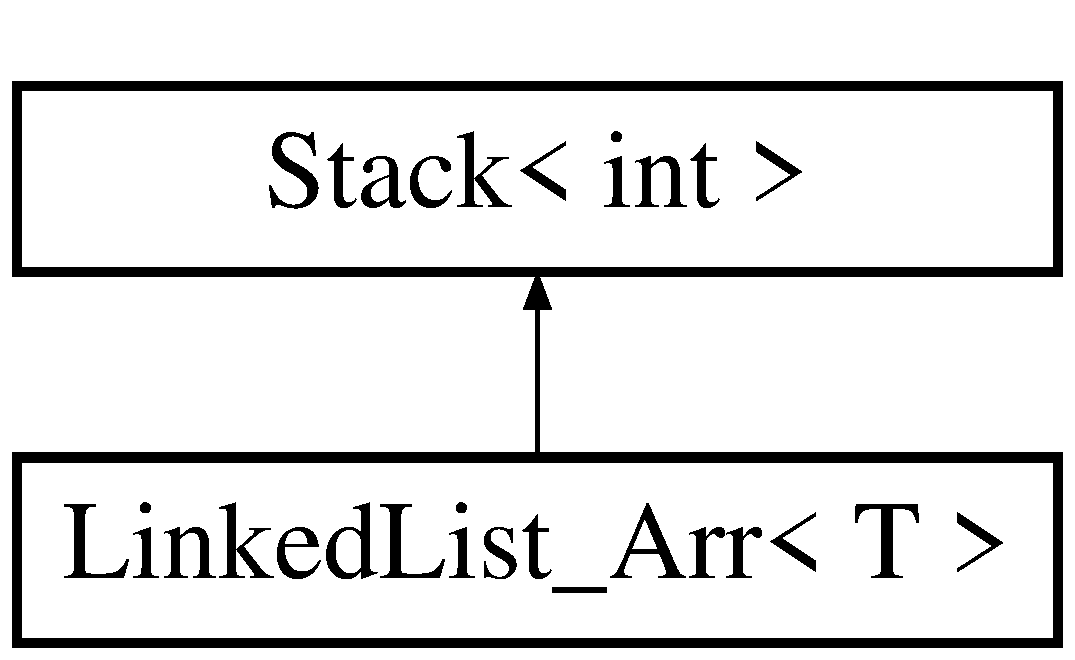
\includegraphics[height=2.000000cm]{class_linked_list___arr}
\end{center}
\end{figure}
\subsection*{Public Member Functions}
\begin{DoxyCompactItemize}
\item 
\hyperlink{class_linked_list___arr_a913dc6e05c3a3c94bb0ef0be43a1202c}{Linked\-List\-\_\-\-Arr} (int \hyperlink{class_linked_list___arr_a52b5c93d6141eb728e60e744c22a06b7}{size})
\item 
\hyperlink{class_linked_list___arr_ad4713d029be52b6cfcd14a0558f12ced}{$\sim$\-Linked\-List\-\_\-\-Arr} ()
\item 
bool \hyperlink{class_linked_list___arr_ac3741a20c72a97e6b37337ba882d9dad}{is\-Off} ()
\item 
T \hyperlink{class_linked_list___arr_a7084841d8f7d76312860d360ff366f20}{item} ()
\item 
void \hyperlink{class_linked_list___arr_a173f5d2e3f4d631b861bbeb9ac674a57}{start} ()
\item 
void \hyperlink{class_linked_list___arr_a034426b6a41088ad772599358e3cec96}{forth} ()
\item 
void \hyperlink{class_linked_list___arr_a317c3d744519ad9036008fcd79e604ee}{insert\-Before} (T data)
\item 
void \hyperlink{class_linked_list___arr_af008582dc60cabeea08e3cac98e0d793}{remove\-At} ()
\item 
void \hyperlink{class_linked_list___arr_a77f9a7fbe17c58df9137e3da3d3f73cd}{whole} ()
\item 
int \& \hyperlink{class_linked_list___arr_a52b5c93d6141eb728e60e744c22a06b7}{size} ()
\item 
int \& \hyperlink{class_linked_list___arr_a5c8bb3dbdc03d6e473142641852bb670}{Get\-\_\-\-Size} ()
\end{DoxyCompactItemize}
\subsection*{Protected Attributes}
\begin{DoxyCompactItemize}
\item 
int \hyperlink{class_linked_list___arr_a9a792afdd7f903981f7ed21aa2239dfd}{head}
\item 
int \hyperlink{class_linked_list___arr_af47d4c0cf43f44120bc658d5d1917f53}{iteratos\-Pos}
\item 
int \hyperlink{class_linked_list___arr_aab0f6d9da0106d51d39048b2f21cf76a}{previous}
\end{DoxyCompactItemize}


\subsection{Constructor \& Destructor Documentation}
\hypertarget{class_linked_list___arr_a913dc6e05c3a3c94bb0ef0be43a1202c}{\index{Linked\-List\-\_\-\-Arr@{Linked\-List\-\_\-\-Arr}!Linked\-List\-\_\-\-Arr@{Linked\-List\-\_\-\-Arr}}
\index{Linked\-List\-\_\-\-Arr@{Linked\-List\-\_\-\-Arr}!LinkedList_Arr@{Linked\-List\-\_\-\-Arr}}
\subsubsection[{Linked\-List\-\_\-\-Arr}]{\setlength{\rightskip}{0pt plus 5cm}template$<$class T $>$ {\bf Linked\-List\-\_\-\-Arr}$<$ T $>$\-::{\bf Linked\-List\-\_\-\-Arr} (
\begin{DoxyParamCaption}
\item[{int}]{size}
\end{DoxyParamCaption}
)}}\label{class_linked_list___arr_a913dc6e05c3a3c94bb0ef0be43a1202c}
\hypertarget{class_linked_list___arr_ad4713d029be52b6cfcd14a0558f12ced}{\index{Linked\-List\-\_\-\-Arr@{Linked\-List\-\_\-\-Arr}!$\sim$\-Linked\-List\-\_\-\-Arr@{$\sim$\-Linked\-List\-\_\-\-Arr}}
\index{$\sim$\-Linked\-List\-\_\-\-Arr@{$\sim$\-Linked\-List\-\_\-\-Arr}!LinkedList_Arr@{Linked\-List\-\_\-\-Arr}}
\subsubsection[{$\sim$\-Linked\-List\-\_\-\-Arr}]{\setlength{\rightskip}{0pt plus 5cm}template$<$class T $>$ {\bf Linked\-List\-\_\-\-Arr}$<$ T $>$\-::$\sim${\bf Linked\-List\-\_\-\-Arr} (
\begin{DoxyParamCaption}
{}
\end{DoxyParamCaption}
)}}\label{class_linked_list___arr_ad4713d029be52b6cfcd14a0558f12ced}


\subsection{Member Function Documentation}
\hypertarget{class_linked_list___arr_a034426b6a41088ad772599358e3cec96}{\index{Linked\-List\-\_\-\-Arr@{Linked\-List\-\_\-\-Arr}!forth@{forth}}
\index{forth@{forth}!LinkedList_Arr@{Linked\-List\-\_\-\-Arr}}
\subsubsection[{forth}]{\setlength{\rightskip}{0pt plus 5cm}template$<$class T $>$ void {\bf Linked\-List\-\_\-\-Arr}$<$ T $>$\-::forth (
\begin{DoxyParamCaption}
{}
\end{DoxyParamCaption}
)}}\label{class_linked_list___arr_a034426b6a41088ad772599358e3cec96}
$\ast$\-Lets iterator\-Pos to take a step forward in the list \hypertarget{class_linked_list___arr_a5c8bb3dbdc03d6e473142641852bb670}{\index{Linked\-List\-\_\-\-Arr@{Linked\-List\-\_\-\-Arr}!Get\-\_\-\-Size@{Get\-\_\-\-Size}}
\index{Get\-\_\-\-Size@{Get\-\_\-\-Size}!LinkedList_Arr@{Linked\-List\-\_\-\-Arr}}
\subsubsection[{Get\-\_\-\-Size}]{\setlength{\rightskip}{0pt plus 5cm}template$<$class T $>$ int \& {\bf Linked\-List\-\_\-\-Arr}$<$ T $>$\-::Get\-\_\-\-Size (
\begin{DoxyParamCaption}
{}
\end{DoxyParamCaption}
)}}\label{class_linked_list___arr_a5c8bb3dbdc03d6e473142641852bb670}
$\ast$\-Function for unit tester \hypertarget{class_linked_list___arr_a317c3d744519ad9036008fcd79e604ee}{\index{Linked\-List\-\_\-\-Arr@{Linked\-List\-\_\-\-Arr}!insert\-Before@{insert\-Before}}
\index{insert\-Before@{insert\-Before}!LinkedList_Arr@{Linked\-List\-\_\-\-Arr}}
\subsubsection[{insert\-Before}]{\setlength{\rightskip}{0pt plus 5cm}template$<$class T $>$ void {\bf Linked\-List\-\_\-\-Arr}$<$ T $>$\-::insert\-Before (
\begin{DoxyParamCaption}
\item[{T}]{data}
\end{DoxyParamCaption}
)}}\label{class_linked_list___arr_a317c3d744519ad9036008fcd79e604ee}
$\ast$\-Gets an index from free\-\_\-nodes and sets the value $\ast$\-If free\-\_\-nodes is empty the \hyperlink{class_stack}{Stack} throws a range\-\_\-error and this method catches it \hypertarget{class_linked_list___arr_ac3741a20c72a97e6b37337ba882d9dad}{\index{Linked\-List\-\_\-\-Arr@{Linked\-List\-\_\-\-Arr}!is\-Off@{is\-Off}}
\index{is\-Off@{is\-Off}!LinkedList_Arr@{Linked\-List\-\_\-\-Arr}}
\subsubsection[{is\-Off}]{\setlength{\rightskip}{0pt plus 5cm}template$<$class T $>$ bool {\bf Linked\-List\-\_\-\-Arr}$<$ T $>$\-::is\-Off (
\begin{DoxyParamCaption}
{}
\end{DoxyParamCaption}
)}}\label{class_linked_list___arr_ac3741a20c72a97e6b37337ba882d9dad}
$\ast$\-Checks if iterator\-Pos == -\/1  true/false \hypertarget{class_linked_list___arr_a7084841d8f7d76312860d360ff366f20}{\index{Linked\-List\-\_\-\-Arr@{Linked\-List\-\_\-\-Arr}!item@{item}}
\index{item@{item}!LinkedList_Arr@{Linked\-List\-\_\-\-Arr}}
\subsubsection[{item}]{\setlength{\rightskip}{0pt plus 5cm}template$<$class T $>$ T {\bf Linked\-List\-\_\-\-Arr}$<$ T $>$\-::item (
\begin{DoxyParamCaption}
{}
\end{DoxyParamCaption}
)}}\label{class_linked_list___arr_a7084841d8f7d76312860d360ff366f20}
$\ast$\-Cheks \hyperlink{class_linked_list___arr_ac3741a20c72a97e6b37337ba882d9dad}{is\-Off()} if iterator\-Pos is -\/1  data if false $\ast$\-Throws a std\-::range\-\_\-error if true \hypertarget{class_linked_list___arr_af008582dc60cabeea08e3cac98e0d793}{\index{Linked\-List\-\_\-\-Arr@{Linked\-List\-\_\-\-Arr}!remove\-At@{remove\-At}}
\index{remove\-At@{remove\-At}!LinkedList_Arr@{Linked\-List\-\_\-\-Arr}}
\subsubsection[{remove\-At}]{\setlength{\rightskip}{0pt plus 5cm}template$<$class T $>$ void {\bf Linked\-List\-\_\-\-Arr}$<$ T $>$\-::remove\-At (
\begin{DoxyParamCaption}
{}
\end{DoxyParamCaption}
)}}\label{class_linked_list___arr_af008582dc60cabeea08e3cac98e0d793}
$\ast$\-Removes the data from the \hyperlink{struct_node}{Node} that iterator\-Pos is \char`\"{}pointing to\char`\"{} \hypertarget{class_linked_list___arr_a52b5c93d6141eb728e60e744c22a06b7}{\index{Linked\-List\-\_\-\-Arr@{Linked\-List\-\_\-\-Arr}!size@{size}}
\index{size@{size}!LinkedList_Arr@{Linked\-List\-\_\-\-Arr}}
\subsubsection[{size}]{\setlength{\rightskip}{0pt plus 5cm}template$<$class T $>$ int \& {\bf Linked\-List\-\_\-\-Arr}$<$ T $>$\-::size (
\begin{DoxyParamCaption}
{}
\end{DoxyParamCaption}
)}}\label{class_linked_list___arr_a52b5c93d6141eb728e60e744c22a06b7}
$\ast$\-Garbage \hypertarget{class_linked_list___arr_a173f5d2e3f4d631b861bbeb9ac674a57}{\index{Linked\-List\-\_\-\-Arr@{Linked\-List\-\_\-\-Arr}!start@{start}}
\index{start@{start}!LinkedList_Arr@{Linked\-List\-\_\-\-Arr}}
\subsubsection[{start}]{\setlength{\rightskip}{0pt plus 5cm}template$<$class T $>$ void {\bf Linked\-List\-\_\-\-Arr}$<$ T $>$\-::start (
\begin{DoxyParamCaption}
{}
\end{DoxyParamCaption}
)}}\label{class_linked_list___arr_a173f5d2e3f4d631b861bbeb9ac674a57}
$\ast$\-Sets iterator\-Pos = head $\ast$\-Sets previous = -\/1 \hypertarget{class_linked_list___arr_a77f9a7fbe17c58df9137e3da3d3f73cd}{\index{Linked\-List\-\_\-\-Arr@{Linked\-List\-\_\-\-Arr}!whole@{whole}}
\index{whole@{whole}!LinkedList_Arr@{Linked\-List\-\_\-\-Arr}}
\subsubsection[{whole}]{\setlength{\rightskip}{0pt plus 5cm}template$<$class T $>$ void {\bf Linked\-List\-\_\-\-Arr}$<$ T $>$\-::whole (
\begin{DoxyParamCaption}
{}
\end{DoxyParamCaption}
)}}\label{class_linked_list___arr_a77f9a7fbe17c58df9137e3da3d3f73cd}
$\ast$\-Garbage method to return all values in the array 

\subsection{Member Data Documentation}
\hypertarget{class_linked_list___arr_a9a792afdd7f903981f7ed21aa2239dfd}{\index{Linked\-List\-\_\-\-Arr@{Linked\-List\-\_\-\-Arr}!head@{head}}
\index{head@{head}!LinkedList_Arr@{Linked\-List\-\_\-\-Arr}}
\subsubsection[{head}]{\setlength{\rightskip}{0pt plus 5cm}template$<$class T$>$ int {\bf Linked\-List\-\_\-\-Arr}$<$ T $>$\-::head\hspace{0.3cm}{\ttfamily [protected]}}}\label{class_linked_list___arr_a9a792afdd7f903981f7ed21aa2239dfd}
\hypertarget{class_linked_list___arr_af47d4c0cf43f44120bc658d5d1917f53}{\index{Linked\-List\-\_\-\-Arr@{Linked\-List\-\_\-\-Arr}!iteratos\-Pos@{iteratos\-Pos}}
\index{iteratos\-Pos@{iteratos\-Pos}!LinkedList_Arr@{Linked\-List\-\_\-\-Arr}}
\subsubsection[{iteratos\-Pos}]{\setlength{\rightskip}{0pt plus 5cm}template$<$class T$>$ int {\bf Linked\-List\-\_\-\-Arr}$<$ T $>$\-::iteratos\-Pos\hspace{0.3cm}{\ttfamily [protected]}}}\label{class_linked_list___arr_af47d4c0cf43f44120bc658d5d1917f53}
\hypertarget{class_linked_list___arr_aab0f6d9da0106d51d39048b2f21cf76a}{\index{Linked\-List\-\_\-\-Arr@{Linked\-List\-\_\-\-Arr}!previous@{previous}}
\index{previous@{previous}!LinkedList_Arr@{Linked\-List\-\_\-\-Arr}}
\subsubsection[{previous}]{\setlength{\rightskip}{0pt plus 5cm}template$<$class T$>$ int {\bf Linked\-List\-\_\-\-Arr}$<$ T $>$\-::previous\hspace{0.3cm}{\ttfamily [protected]}}}\label{class_linked_list___arr_aab0f6d9da0106d51d39048b2f21cf76a}


The documentation for this class was generated from the following file\-:\begin{DoxyCompactItemize}
\item 
//afs/ltu.\-se/students/all/ponste-\/5/\-My Documents/\-Programmering\-\_\-\-Labbar/\-D0041\-D/\-Labb01/\-Linked\-List/\hyperlink{_array__v2_8h}{Array\-\_\-v2.\-h}\end{DoxyCompactItemize}

\hypertarget{class_l_ltester}{\section{L\-Ltester$<$ T $>$ Class Template Reference}
\label{class_l_ltester}\index{L\-Ltester$<$ T $>$@{L\-Ltester$<$ T $>$}}
}


{\ttfamily \#include $<$Unit\-\_\-test.\-h$>$}

\subsection*{Public Member Functions}
\begin{DoxyCompactItemize}
\item 
void \hyperlink{class_l_ltester_af16564815500d55d820f996b9bfd73e4}{Add} (\hyperlink{class_linked_list}{Linked\-List} \&ll, T value)
\item 
void \hyperlink{class_l_ltester_ade176cb3006c4e1a3806abfa0378ecae}{Add} (\hyperlink{class_linked_list___arr}{Linked\-List\-\_\-\-Arr}$<$ T $>$ \&la, T value)
\item 
void \hyperlink{class_l_ltester_aa60fe27492ab311d316ac75c02ee95c1}{Add} (\hyperlink{class_stack}{Stack}$<$ T $>$ \&stack, T value)
\item 
void \hyperlink{class_l_ltester_af0a2eb223e399c33bb169108e838f85a}{Add} (\hyperlink{class_queue}{Queue}$<$ T $>$ \&que, T value)
\item 
void \hyperlink{class_l_ltester_a5c7cfb2fab433e1b91d49ef63fe63c97}{Delete} (\hyperlink{class_linked_list}{Linked\-List} \&ll)
\item 
void \hyperlink{class_l_ltester_ad8b9ca486cc9df214e8b1839f08eb29e}{Delete} (\hyperlink{class_linked_list___arr}{Linked\-List\-\_\-\-Arr}$<$ T $>$ \&la)
\item 
void \hyperlink{class_l_ltester_a96be238835f40dad4af79ce19f676591}{Delete} (\hyperlink{class_stack}{Stack}$<$ T $>$ \&stack)
\item 
void \hyperlink{class_l_ltester_ac88a926ffe302d4e2a4e263814adcd3e}{Delete} (\hyperlink{class_queue}{Queue}$<$ T $>$ \&que)
\item 
void \hyperlink{class_l_ltester_accd88a631a2a4fcb7d0d00f306e2b649}{Start} (\hyperlink{class_linked_list}{Linked\-List} \&ll)
\item 
void \hyperlink{class_l_ltester_a6b070aa9405668456e6aaf43986677ca}{Start} (\hyperlink{class_linked_list___arr}{Linked\-List\-\_\-\-Arr}$<$ T $>$ \&la)
\item 
void \hyperlink{class_l_ltester_a9a4fc66335b0f355ce846bddb1ea38c2}{Step} (\hyperlink{class_linked_list}{Linked\-List} \&ll)
\item 
void \hyperlink{class_l_ltester_a0f2fa22f42f7217700c95dfb223689dd}{Step} (\hyperlink{class_linked_list___arr}{Linked\-List\-\_\-\-Arr}$<$ T $>$ \&la)
\item 
void \hyperlink{class_l_ltester_abae4772e90c34c509de01c9d1210cdc8}{Get} (\hyperlink{class_linked_list}{Linked\-List} \&ll)
\item 
void \hyperlink{class_l_ltester_abf6915fe5a976213848e60c1f8ce4d3f}{Get} (\hyperlink{class_linked_list___arr}{Linked\-List\-\_\-\-Arr}$<$ T $>$ \&la)
\item 
void \hyperlink{class_l_ltester_a608b153b3d91bd514cda7473af9a79e4}{Get} (\hyperlink{class_stack}{Stack}$<$ T $>$ \&stack)
\item 
void \hyperlink{class_l_ltester_a653c5ffda0d3d4a21766e0fe29286ac6}{Get} (\hyperlink{class_queue}{Queue}$<$ T $>$ \&que)
\item 
void \hyperlink{class_l_ltester_af1e7da6a3dd01b624e5c29b4faa87ffd}{Add\-\_\-\-Beginning} (\hyperlink{class_linked_list}{Linked\-List} \&ll, T value)
\item 
void \hyperlink{class_l_ltester_aa7f798f129a87f11b37527991f3d0da5}{Add\-\_\-\-Beginning} (\hyperlink{class_linked_list___arr}{Linked\-List\-\_\-\-Arr}$<$ T $>$ \&la, T value)
\item 
void \hyperlink{class_l_ltester_ad3c123934e61077648920eaa34e665d2}{Add\-\_\-\-More} (\hyperlink{class_linked_list___arr}{Linked\-List\-\_\-\-Arr}$<$ T $>$ \&la, T value)
\item 
void \hyperlink{class_l_ltester_a70219340c04d3aa476897209b7d75740}{Delete\-\_\-\-Beginning} (\hyperlink{class_linked_list}{Linked\-List} \&ll)
\item 
void \hyperlink{class_l_ltester_a8ed774e316f8f218aa0f75c783e25d25}{Delete\-\_\-\-Beginning} (\hyperlink{class_linked_list___arr}{Linked\-List\-\_\-\-Arr}$<$ T $>$ \&la)
\item 
void \hyperlink{class_l_ltester_a29aa03d43d14bf3d066531dd984ea8c3}{Step\-\_\-\-Test} (\hyperlink{class_linked_list}{Linked\-List} \&ll)
\item 
void \hyperlink{class_l_ltester_ab10a3a7f3eb182e9b3feaeb7c368d9a4}{Step\-\_\-\-Test} (\hyperlink{class_linked_list___arr}{Linked\-List\-\_\-\-Arr}$<$ T $>$ \&la)
\item 
void \hyperlink{class_l_ltester_a01df83a371999cccb2d422839373c538}{Delete\-\_\-\-All} (\hyperlink{class_linked_list}{Linked\-List} \&ll)
\item 
void \hyperlink{class_l_ltester_a86b0a4f1c87b4db73e965141126aa425}{Delete\-\_\-\-All} (\hyperlink{class_linked_list___arr}{Linked\-List\-\_\-\-Arr}$<$ T $>$ \&la)
\item 
void \hyperlink{class_l_ltester_aa669cffc9af3f0af3f7af2a42079b555}{Delete\-\_\-\-All} (\hyperlink{class_stack}{Stack}$<$ T $>$ \&stack)
\item 
void \hyperlink{class_l_ltester_a6b4b5fc311e0daabf2605493ee1c0d70}{Delete\-\_\-\-All} (\hyperlink{class_queue}{Queue}$<$ T $>$ \&que)
\item 
void \hyperlink{class_l_ltester_aa8fd00f85de53957afd4d1306af17fa0}{Start\-\_\-\-Test} (\hyperlink{class_linked_list}{Linked\-List} \&ll)
\item 
void \hyperlink{class_l_ltester_a85f069982d814a755412c83237d2dc38}{Start\-\_\-\-Test} (\hyperlink{class_linked_list___arr}{Linked\-List\-\_\-\-Arr}$<$ T $>$ \&la)
\item 
void \hyperlink{class_l_ltester_a8046a64f9635a09b6b74a86ad6840b9c}{Start\-\_\-\-Test} (\hyperlink{class_stack}{Stack}$<$ T $>$ \&stack)
\item 
void \hyperlink{class_l_ltester_a971c6ec6596cf580f74dd286abe75c8f}{Start\-\_\-\-Test} (\hyperlink{class_queue}{Queue}$<$ T $>$ \&que)
\end{DoxyCompactItemize}


\subsection{Member Function Documentation}
\hypertarget{class_l_ltester_af16564815500d55d820f996b9bfd73e4}{\index{L\-Ltester@{L\-Ltester}!Add@{Add}}
\index{Add@{Add}!LLtester@{L\-Ltester}}
\subsubsection[{Add}]{\setlength{\rightskip}{0pt plus 5cm}template$<$class T $>$ void {\bf L\-Ltester}$<$ T $>$\-::Add (
\begin{DoxyParamCaption}
\item[{{\bf Linked\-List} \&}]{ll, }
\item[{T}]{value}
\end{DoxyParamCaption}
)}}\label{class_l_ltester_af16564815500d55d820f996b9bfd73e4}
$\ast$\-Adds a number between 0-\/$>$value except for \hyperlink{class_linked_list___arr}{Linked\-List\-\_\-\-Arr} \hypertarget{class_l_ltester_ade176cb3006c4e1a3806abfa0378ecae}{\index{L\-Ltester@{L\-Ltester}!Add@{Add}}
\index{Add@{Add}!LLtester@{L\-Ltester}}
\subsubsection[{Add}]{\setlength{\rightskip}{0pt plus 5cm}template$<$class T $>$ void {\bf L\-Ltester}$<$ T $>$\-::Add (
\begin{DoxyParamCaption}
\item[{{\bf Linked\-List\-\_\-\-Arr}$<$ T $>$ \&}]{la, }
\item[{T}]{value}
\end{DoxyParamCaption}
)}}\label{class_l_ltester_ade176cb3006c4e1a3806abfa0378ecae}
\hypertarget{class_l_ltester_aa60fe27492ab311d316ac75c02ee95c1}{\index{L\-Ltester@{L\-Ltester}!Add@{Add}}
\index{Add@{Add}!LLtester@{L\-Ltester}}
\subsubsection[{Add}]{\setlength{\rightskip}{0pt plus 5cm}template$<$class T $>$ void {\bf L\-Ltester}$<$ T $>$\-::Add (
\begin{DoxyParamCaption}
\item[{{\bf Stack}$<$ T $>$ \&}]{stack, }
\item[{T}]{value}
\end{DoxyParamCaption}
)}}\label{class_l_ltester_aa60fe27492ab311d316ac75c02ee95c1}
\hypertarget{class_l_ltester_af0a2eb223e399c33bb169108e838f85a}{\index{L\-Ltester@{L\-Ltester}!Add@{Add}}
\index{Add@{Add}!LLtester@{L\-Ltester}}
\subsubsection[{Add}]{\setlength{\rightskip}{0pt plus 5cm}template$<$class T $>$ void {\bf L\-Ltester}$<$ T $>$\-::Add (
\begin{DoxyParamCaption}
\item[{{\bf Queue}$<$ T $>$ \&}]{que, }
\item[{T}]{value}
\end{DoxyParamCaption}
)}}\label{class_l_ltester_af0a2eb223e399c33bb169108e838f85a}
\hypertarget{class_l_ltester_af1e7da6a3dd01b624e5c29b4faa87ffd}{\index{L\-Ltester@{L\-Ltester}!Add\-\_\-\-Beginning@{Add\-\_\-\-Beginning}}
\index{Add\-\_\-\-Beginning@{Add\-\_\-\-Beginning}!LLtester@{L\-Ltester}}
\subsubsection[{Add\-\_\-\-Beginning}]{\setlength{\rightskip}{0pt plus 5cm}template$<$class T $>$ void {\bf L\-Ltester}$<$ T $>$\-::Add\-\_\-\-Beginning (
\begin{DoxyParamCaption}
\item[{{\bf Linked\-List} \&}]{ll, }
\item[{T}]{value}
\end{DoxyParamCaption}
)}}\label{class_l_ltester_af1e7da6a3dd01b624e5c29b4faa87ffd}
$\ast$tries adds a value to the beginning \hypertarget{class_l_ltester_aa7f798f129a87f11b37527991f3d0da5}{\index{L\-Ltester@{L\-Ltester}!Add\-\_\-\-Beginning@{Add\-\_\-\-Beginning}}
\index{Add\-\_\-\-Beginning@{Add\-\_\-\-Beginning}!LLtester@{L\-Ltester}}
\subsubsection[{Add\-\_\-\-Beginning}]{\setlength{\rightskip}{0pt plus 5cm}template$<$class T $>$ void {\bf L\-Ltester}$<$ T $>$\-::Add\-\_\-\-Beginning (
\begin{DoxyParamCaption}
\item[{{\bf Linked\-List\-\_\-\-Arr}$<$ T $>$ \&}]{la, }
\item[{T}]{value}
\end{DoxyParamCaption}
)}}\label{class_l_ltester_aa7f798f129a87f11b37527991f3d0da5}
\hypertarget{class_l_ltester_ad3c123934e61077648920eaa34e665d2}{\index{L\-Ltester@{L\-Ltester}!Add\-\_\-\-More@{Add\-\_\-\-More}}
\index{Add\-\_\-\-More@{Add\-\_\-\-More}!LLtester@{L\-Ltester}}
\subsubsection[{Add\-\_\-\-More}]{\setlength{\rightskip}{0pt plus 5cm}template$<$class T $>$ void {\bf L\-Ltester}$<$ T $>$\-::Add\-\_\-\-More (
\begin{DoxyParamCaption}
\item[{{\bf Linked\-List\-\_\-\-Arr}$<$ T $>$ \&}]{la, }
\item[{T}]{value}
\end{DoxyParamCaption}
)}}\label{class_l_ltester_ad3c123934e61077648920eaa34e665d2}
\hypertarget{class_l_ltester_a5c7cfb2fab433e1b91d49ef63fe63c97}{\index{L\-Ltester@{L\-Ltester}!Delete@{Delete}}
\index{Delete@{Delete}!LLtester@{L\-Ltester}}
\subsubsection[{Delete}]{\setlength{\rightskip}{0pt plus 5cm}template$<$class T $>$ void {\bf L\-Ltester}$<$ T $>$\-::Delete (
\begin{DoxyParamCaption}
\item[{{\bf Linked\-List} \&}]{ll}
\end{DoxyParamCaption}
)}}\label{class_l_ltester_a5c7cfb2fab433e1b91d49ef63fe63c97}
$\ast$\-Calls the methods to delete a node \hypertarget{class_l_ltester_ad8b9ca486cc9df214e8b1839f08eb29e}{\index{L\-Ltester@{L\-Ltester}!Delete@{Delete}}
\index{Delete@{Delete}!LLtester@{L\-Ltester}}
\subsubsection[{Delete}]{\setlength{\rightskip}{0pt plus 5cm}template$<$class T $>$ void {\bf L\-Ltester}$<$ T $>$\-::Delete (
\begin{DoxyParamCaption}
\item[{{\bf Linked\-List\-\_\-\-Arr}$<$ T $>$ \&}]{la}
\end{DoxyParamCaption}
)}}\label{class_l_ltester_ad8b9ca486cc9df214e8b1839f08eb29e}
\hypertarget{class_l_ltester_a96be238835f40dad4af79ce19f676591}{\index{L\-Ltester@{L\-Ltester}!Delete@{Delete}}
\index{Delete@{Delete}!LLtester@{L\-Ltester}}
\subsubsection[{Delete}]{\setlength{\rightskip}{0pt plus 5cm}template$<$class T $>$ void {\bf L\-Ltester}$<$ T $>$\-::Delete (
\begin{DoxyParamCaption}
\item[{{\bf Stack}$<$ T $>$ \&}]{stack}
\end{DoxyParamCaption}
)}}\label{class_l_ltester_a96be238835f40dad4af79ce19f676591}
\hypertarget{class_l_ltester_ac88a926ffe302d4e2a4e263814adcd3e}{\index{L\-Ltester@{L\-Ltester}!Delete@{Delete}}
\index{Delete@{Delete}!LLtester@{L\-Ltester}}
\subsubsection[{Delete}]{\setlength{\rightskip}{0pt plus 5cm}template$<$class T $>$ void {\bf L\-Ltester}$<$ T $>$\-::Delete (
\begin{DoxyParamCaption}
\item[{{\bf Queue}$<$ T $>$ \&}]{que}
\end{DoxyParamCaption}
)}}\label{class_l_ltester_ac88a926ffe302d4e2a4e263814adcd3e}
\hypertarget{class_l_ltester_a01df83a371999cccb2d422839373c538}{\index{L\-Ltester@{L\-Ltester}!Delete\-\_\-\-All@{Delete\-\_\-\-All}}
\index{Delete\-\_\-\-All@{Delete\-\_\-\-All}!LLtester@{L\-Ltester}}
\subsubsection[{Delete\-\_\-\-All}]{\setlength{\rightskip}{0pt plus 5cm}template$<$class T $>$ void {\bf L\-Ltester}$<$ T $>$\-::Delete\-\_\-\-All (
\begin{DoxyParamCaption}
\item[{{\bf Linked\-List} \&}]{ll}
\end{DoxyParamCaption}
)}}\label{class_l_ltester_a01df83a371999cccb2d422839373c538}
$\ast$\-Deletes all nodes +1 to see what happens 
\begin{DoxyParams}{Parameters}
{\em takes} & a class of the same type as argument \\
\hline
\end{DoxyParams}
\hypertarget{class_l_ltester_a86b0a4f1c87b4db73e965141126aa425}{\index{L\-Ltester@{L\-Ltester}!Delete\-\_\-\-All@{Delete\-\_\-\-All}}
\index{Delete\-\_\-\-All@{Delete\-\_\-\-All}!LLtester@{L\-Ltester}}
\subsubsection[{Delete\-\_\-\-All}]{\setlength{\rightskip}{0pt plus 5cm}template$<$class T $>$ void {\bf L\-Ltester}$<$ T $>$\-::Delete\-\_\-\-All (
\begin{DoxyParamCaption}
\item[{{\bf Linked\-List\-\_\-\-Arr}$<$ T $>$ \&}]{la}
\end{DoxyParamCaption}
)}}\label{class_l_ltester_a86b0a4f1c87b4db73e965141126aa425}
\hypertarget{class_l_ltester_aa669cffc9af3f0af3f7af2a42079b555}{\index{L\-Ltester@{L\-Ltester}!Delete\-\_\-\-All@{Delete\-\_\-\-All}}
\index{Delete\-\_\-\-All@{Delete\-\_\-\-All}!LLtester@{L\-Ltester}}
\subsubsection[{Delete\-\_\-\-All}]{\setlength{\rightskip}{0pt plus 5cm}template$<$class T $>$ void {\bf L\-Ltester}$<$ T $>$\-::Delete\-\_\-\-All (
\begin{DoxyParamCaption}
\item[{{\bf Stack}$<$ T $>$ \&}]{stack}
\end{DoxyParamCaption}
)}}\label{class_l_ltester_aa669cffc9af3f0af3f7af2a42079b555}
\hypertarget{class_l_ltester_a6b4b5fc311e0daabf2605493ee1c0d70}{\index{L\-Ltester@{L\-Ltester}!Delete\-\_\-\-All@{Delete\-\_\-\-All}}
\index{Delete\-\_\-\-All@{Delete\-\_\-\-All}!LLtester@{L\-Ltester}}
\subsubsection[{Delete\-\_\-\-All}]{\setlength{\rightskip}{0pt plus 5cm}template$<$class T $>$ void {\bf L\-Ltester}$<$ T $>$\-::Delete\-\_\-\-All (
\begin{DoxyParamCaption}
\item[{{\bf Queue}$<$ T $>$ \&}]{que}
\end{DoxyParamCaption}
)}}\label{class_l_ltester_a6b4b5fc311e0daabf2605493ee1c0d70}
\hypertarget{class_l_ltester_a70219340c04d3aa476897209b7d75740}{\index{L\-Ltester@{L\-Ltester}!Delete\-\_\-\-Beginning@{Delete\-\_\-\-Beginning}}
\index{Delete\-\_\-\-Beginning@{Delete\-\_\-\-Beginning}!LLtester@{L\-Ltester}}
\subsubsection[{Delete\-\_\-\-Beginning}]{\setlength{\rightskip}{0pt plus 5cm}template$<$class T $>$ void {\bf L\-Ltester}$<$ T $>$\-::Delete\-\_\-\-Beginning (
\begin{DoxyParamCaption}
\item[{{\bf Linked\-List} \&}]{ll}
\end{DoxyParamCaption}
)}}\label{class_l_ltester_a70219340c04d3aa476897209b7d75740}
$\ast$\-Goes to the beginning and try to delete that \hyperlink{struct_node}{Node} 
\begin{DoxyParams}{Parameters}
{\em takes} & a \hyperlink{class_linked_list}{Linked\-List} or \hyperlink{class_linked_list___arr}{Linked\-List\-\_\-\-Arr} as argument $\ast$\-Linked\-List\-\_\-\-Arr must be of the same type as \hyperlink{class_l_ltester}{L\-Ltester} \\
\hline
\end{DoxyParams}
\hypertarget{class_l_ltester_a8ed774e316f8f218aa0f75c783e25d25}{\index{L\-Ltester@{L\-Ltester}!Delete\-\_\-\-Beginning@{Delete\-\_\-\-Beginning}}
\index{Delete\-\_\-\-Beginning@{Delete\-\_\-\-Beginning}!LLtester@{L\-Ltester}}
\subsubsection[{Delete\-\_\-\-Beginning}]{\setlength{\rightskip}{0pt plus 5cm}template$<$class T $>$ void {\bf L\-Ltester}$<$ T $>$\-::Delete\-\_\-\-Beginning (
\begin{DoxyParamCaption}
\item[{{\bf Linked\-List\-\_\-\-Arr}$<$ T $>$ \&}]{la}
\end{DoxyParamCaption}
)}}\label{class_l_ltester_a8ed774e316f8f218aa0f75c783e25d25}
\hypertarget{class_l_ltester_abae4772e90c34c509de01c9d1210cdc8}{\index{L\-Ltester@{L\-Ltester}!Get@{Get}}
\index{Get@{Get}!LLtester@{L\-Ltester}}
\subsubsection[{Get}]{\setlength{\rightskip}{0pt plus 5cm}template$<$class T $>$ void {\bf L\-Ltester}$<$ T $>$\-::Get (
\begin{DoxyParamCaption}
\item[{{\bf Linked\-List} \&}]{ll}
\end{DoxyParamCaption}
)}}\label{class_l_ltester_abae4772e90c34c509de01c9d1210cdc8}
$\ast$\-Prints out the value returned from each class. \hypertarget{class_l_ltester_abf6915fe5a976213848e60c1f8ce4d3f}{\index{L\-Ltester@{L\-Ltester}!Get@{Get}}
\index{Get@{Get}!LLtester@{L\-Ltester}}
\subsubsection[{Get}]{\setlength{\rightskip}{0pt plus 5cm}template$<$class T $>$ void {\bf L\-Ltester}$<$ T $>$\-::Get (
\begin{DoxyParamCaption}
\item[{{\bf Linked\-List\-\_\-\-Arr}$<$ T $>$ \&}]{la}
\end{DoxyParamCaption}
)}}\label{class_l_ltester_abf6915fe5a976213848e60c1f8ce4d3f}
\hypertarget{class_l_ltester_a608b153b3d91bd514cda7473af9a79e4}{\index{L\-Ltester@{L\-Ltester}!Get@{Get}}
\index{Get@{Get}!LLtester@{L\-Ltester}}
\subsubsection[{Get}]{\setlength{\rightskip}{0pt plus 5cm}template$<$class T $>$ void {\bf L\-Ltester}$<$ T $>$\-::Get (
\begin{DoxyParamCaption}
\item[{{\bf Stack}$<$ T $>$ \&}]{stack}
\end{DoxyParamCaption}
)}}\label{class_l_ltester_a608b153b3d91bd514cda7473af9a79e4}
\hypertarget{class_l_ltester_a653c5ffda0d3d4a21766e0fe29286ac6}{\index{L\-Ltester@{L\-Ltester}!Get@{Get}}
\index{Get@{Get}!LLtester@{L\-Ltester}}
\subsubsection[{Get}]{\setlength{\rightskip}{0pt plus 5cm}template$<$class T $>$ void {\bf L\-Ltester}$<$ T $>$\-::Get (
\begin{DoxyParamCaption}
\item[{{\bf Queue}$<$ T $>$ \&}]{que}
\end{DoxyParamCaption}
)}}\label{class_l_ltester_a653c5ffda0d3d4a21766e0fe29286ac6}
\hypertarget{class_l_ltester_accd88a631a2a4fcb7d0d00f306e2b649}{\index{L\-Ltester@{L\-Ltester}!Start@{Start}}
\index{Start@{Start}!LLtester@{L\-Ltester}}
\subsubsection[{Start}]{\setlength{\rightskip}{0pt plus 5cm}template$<$class T $>$ void {\bf L\-Ltester}$<$ T $>$\-::Start (
\begin{DoxyParamCaption}
\item[{{\bf Linked\-List} \&}]{ll}
\end{DoxyParamCaption}
)}}\label{class_l_ltester_accd88a631a2a4fcb7d0d00f306e2b649}
$\ast$\-Method to set iterator\-Pos to the beginning of the list \hypertarget{class_l_ltester_a6b070aa9405668456e6aaf43986677ca}{\index{L\-Ltester@{L\-Ltester}!Start@{Start}}
\index{Start@{Start}!LLtester@{L\-Ltester}}
\subsubsection[{Start}]{\setlength{\rightskip}{0pt plus 5cm}template$<$class T $>$ void {\bf L\-Ltester}$<$ T $>$\-::Start (
\begin{DoxyParamCaption}
\item[{{\bf Linked\-List\-\_\-\-Arr}$<$ T $>$ \&}]{la}
\end{DoxyParamCaption}
)}}\label{class_l_ltester_a6b070aa9405668456e6aaf43986677ca}
\hypertarget{class_l_ltester_aa8fd00f85de53957afd4d1306af17fa0}{\index{L\-Ltester@{L\-Ltester}!Start\-\_\-\-Test@{Start\-\_\-\-Test}}
\index{Start\-\_\-\-Test@{Start\-\_\-\-Test}!LLtester@{L\-Ltester}}
\subsubsection[{Start\-\_\-\-Test}]{\setlength{\rightskip}{0pt plus 5cm}template$<$class T $>$ void {\bf L\-Ltester}$<$ T $>$\-::Start\-\_\-\-Test (
\begin{DoxyParamCaption}
\item[{{\bf Linked\-List} \&}]{ll}
\end{DoxyParamCaption}
)}}\label{class_l_ltester_aa8fd00f85de53957afd4d1306af17fa0}
$\ast$\-Test to check most possible errors $\ast$\-Calls Step\-\_\-\-Test, Delete\-\_\-\-All, Add\-\_\-\-Beginning and Get 
\begin{DoxyParams}{Parameters}
{\em takes} & a class of the same type as argument \\
\hline
\end{DoxyParams}
\hypertarget{class_l_ltester_a85f069982d814a755412c83237d2dc38}{\index{L\-Ltester@{L\-Ltester}!Start\-\_\-\-Test@{Start\-\_\-\-Test}}
\index{Start\-\_\-\-Test@{Start\-\_\-\-Test}!LLtester@{L\-Ltester}}
\subsubsection[{Start\-\_\-\-Test}]{\setlength{\rightskip}{0pt plus 5cm}template$<$class T $>$ void {\bf L\-Ltester}$<$ T $>$\-::Start\-\_\-\-Test (
\begin{DoxyParamCaption}
\item[{{\bf Linked\-List\-\_\-\-Arr}$<$ T $>$ \&}]{la}
\end{DoxyParamCaption}
)}}\label{class_l_ltester_a85f069982d814a755412c83237d2dc38}
\hypertarget{class_l_ltester_a8046a64f9635a09b6b74a86ad6840b9c}{\index{L\-Ltester@{L\-Ltester}!Start\-\_\-\-Test@{Start\-\_\-\-Test}}
\index{Start\-\_\-\-Test@{Start\-\_\-\-Test}!LLtester@{L\-Ltester}}
\subsubsection[{Start\-\_\-\-Test}]{\setlength{\rightskip}{0pt plus 5cm}template$<$class T $>$ void {\bf L\-Ltester}$<$ T $>$\-::Start\-\_\-\-Test (
\begin{DoxyParamCaption}
\item[{{\bf Stack}$<$ T $>$ \&}]{stack}
\end{DoxyParamCaption}
)}}\label{class_l_ltester_a8046a64f9635a09b6b74a86ad6840b9c}
\hypertarget{class_l_ltester_a971c6ec6596cf580f74dd286abe75c8f}{\index{L\-Ltester@{L\-Ltester}!Start\-\_\-\-Test@{Start\-\_\-\-Test}}
\index{Start\-\_\-\-Test@{Start\-\_\-\-Test}!LLtester@{L\-Ltester}}
\subsubsection[{Start\-\_\-\-Test}]{\setlength{\rightskip}{0pt plus 5cm}template$<$class T $>$ void {\bf L\-Ltester}$<$ T $>$\-::Start\-\_\-\-Test (
\begin{DoxyParamCaption}
\item[{{\bf Queue}$<$ T $>$ \&}]{que}
\end{DoxyParamCaption}
)}}\label{class_l_ltester_a971c6ec6596cf580f74dd286abe75c8f}
\hypertarget{class_l_ltester_a9a4fc66335b0f355ce846bddb1ea38c2}{\index{L\-Ltester@{L\-Ltester}!Step@{Step}}
\index{Step@{Step}!LLtester@{L\-Ltester}}
\subsubsection[{Step}]{\setlength{\rightskip}{0pt plus 5cm}template$<$class T $>$ void {\bf L\-Ltester}$<$ T $>$\-::Step (
\begin{DoxyParamCaption}
\item[{{\bf Linked\-List} \&}]{ll}
\end{DoxyParamCaption}
)}}\label{class_l_ltester_a9a4fc66335b0f355ce846bddb1ea38c2}
$\ast$\-Lets iterator\-Pos in \hyperlink{class_linked_list}{Linked\-List} and \hyperlink{class_linked_list___arr}{Linked\-List\-\_\-\-Arr} take a step forward in the list \hypertarget{class_l_ltester_a0f2fa22f42f7217700c95dfb223689dd}{\index{L\-Ltester@{L\-Ltester}!Step@{Step}}
\index{Step@{Step}!LLtester@{L\-Ltester}}
\subsubsection[{Step}]{\setlength{\rightskip}{0pt plus 5cm}template$<$class T $>$ void {\bf L\-Ltester}$<$ T $>$\-::Step (
\begin{DoxyParamCaption}
\item[{{\bf Linked\-List\-\_\-\-Arr}$<$ T $>$ \&}]{la}
\end{DoxyParamCaption}
)}}\label{class_l_ltester_a0f2fa22f42f7217700c95dfb223689dd}
\hypertarget{class_l_ltester_a29aa03d43d14bf3d066531dd984ea8c3}{\index{L\-Ltester@{L\-Ltester}!Step\-\_\-\-Test@{Step\-\_\-\-Test}}
\index{Step\-\_\-\-Test@{Step\-\_\-\-Test}!LLtester@{L\-Ltester}}
\subsubsection[{Step\-\_\-\-Test}]{\setlength{\rightskip}{0pt plus 5cm}template$<$class T $>$ void {\bf L\-Ltester}$<$ T $>$\-::Step\-\_\-\-Test (
\begin{DoxyParamCaption}
\item[{{\bf Linked\-List} \&}]{ll}
\end{DoxyParamCaption}
)}}\label{class_l_ltester_a29aa03d43d14bf3d066531dd984ea8c3}
$\ast$\-Calls forth() to the end +1 step  an list of type \hyperlink{class_linked_list}{Linked\-List} or \hyperlink{class_linked_list___arr}{Linked\-List\-\_\-\-Arr} $\ast$$\ast$\-Linked\-List\-\_\-\-Arr must be of the same type as \hyperlink{class_l_ltester}{L\-Ltester} \hypertarget{class_l_ltester_ab10a3a7f3eb182e9b3feaeb7c368d9a4}{\index{L\-Ltester@{L\-Ltester}!Step\-\_\-\-Test@{Step\-\_\-\-Test}}
\index{Step\-\_\-\-Test@{Step\-\_\-\-Test}!LLtester@{L\-Ltester}}
\subsubsection[{Step\-\_\-\-Test}]{\setlength{\rightskip}{0pt plus 5cm}template$<$class T $>$ void {\bf L\-Ltester}$<$ T $>$\-::Step\-\_\-\-Test (
\begin{DoxyParamCaption}
\item[{{\bf Linked\-List\-\_\-\-Arr}$<$ T $>$ \&}]{la}
\end{DoxyParamCaption}
)}}\label{class_l_ltester_ab10a3a7f3eb182e9b3feaeb7c368d9a4}


The documentation for this class was generated from the following file\-:\begin{DoxyCompactItemize}
\item 
//afs/ltu.\-se/students/all/ponste-\/5/\-My Documents/\-Programmering\-\_\-\-Labbar/\-D0041\-D/\-Labb01/\-Linked\-List/\hyperlink{_unit__test_8h}{Unit\-\_\-test.\-h}\end{DoxyCompactItemize}

\hypertarget{struct_node}{\section{Node Struct Reference}
\label{struct_node}\index{Node@{Node}}
}


{\ttfamily \#include $<$Linked\-List.\-h$>$}

\subsection*{Public Member Functions}
\begin{DoxyCompactItemize}
\item 
\hyperlink{struct_node_ad7a34779cad45d997bfd6d3d8043c75f}{Node} ()
\end{DoxyCompactItemize}
\subsection*{Public Attributes}
\begin{DoxyCompactItemize}
\item 
int \hyperlink{struct_node_af5dfeb66f4098a82918aa3af132ac91f}{number}
\item 
\hyperlink{struct_node}{Node} $\ast$ \hyperlink{struct_node_a2559a716f69ccaa76d648d9f1b83065e}{next}
\end{DoxyCompactItemize}


\subsection{Constructor \& Destructor Documentation}
\hypertarget{struct_node_ad7a34779cad45d997bfd6d3d8043c75f}{\index{Node@{Node}!Node@{Node}}
\index{Node@{Node}!Node@{Node}}
\subsubsection[{Node}]{\setlength{\rightskip}{0pt plus 5cm}Node\-::\-Node (
\begin{DoxyParamCaption}
{}
\end{DoxyParamCaption}
)}}\label{struct_node_ad7a34779cad45d997bfd6d3d8043c75f}


\subsection{Member Data Documentation}
\hypertarget{struct_node_a2559a716f69ccaa76d648d9f1b83065e}{\index{Node@{Node}!next@{next}}
\index{next@{next}!Node@{Node}}
\subsubsection[{next}]{\setlength{\rightskip}{0pt plus 5cm}{\bf Node}$\ast$ Node\-::next}}\label{struct_node_a2559a716f69ccaa76d648d9f1b83065e}
\hypertarget{struct_node_af5dfeb66f4098a82918aa3af132ac91f}{\index{Node@{Node}!number@{number}}
\index{number@{number}!Node@{Node}}
\subsubsection[{number}]{\setlength{\rightskip}{0pt plus 5cm}int Node\-::number}}\label{struct_node_af5dfeb66f4098a82918aa3af132ac91f}


The documentation for this struct was generated from the following files\-:\begin{DoxyCompactItemize}
\item 
//afs/ltu.\-se/students/all/ponste-\/5/\-My Documents/\-Programmering\-\_\-\-Labbar/\-D0041\-D/\-Labb01/\-Linked\-List/\hyperlink{_linked_list_8h}{Linked\-List.\-h}\item 
//afs/ltu.\-se/students/all/ponste-\/5/\-My Documents/\-Programmering\-\_\-\-Labbar/\-D0041\-D/\-Labb01/\-Linked\-List/\hyperlink{_linked_list_8cpp}{Linked\-List.\-cpp}\end{DoxyCompactItemize}

\hypertarget{class_queue}{\section{Queue$<$ T $>$ Class Template Reference}
\label{class_queue}\index{Queue$<$ T $>$@{Queue$<$ T $>$}}
}


{\ttfamily \#include $<$Queue.\-h$>$}

\subsection*{Public Member Functions}
\begin{DoxyCompactItemize}
\item 
\hyperlink{class_queue_af73bb29c868f7b37f369c668f114bd9f}{Queue} ()
\item 
\hyperlink{class_queue_aa7eef1b427e24555780505de20e9acbc}{$\sim$\-Queue} ()
\item 
void \hyperlink{class_queue_afd06ea5c60823980cbad3ec8db7a7b5b}{Enqueue} (T in\-\_\-data)
\item 
void \hyperlink{class_queue_aae9f32d812e1c5fccecbfe4dde25a338}{Dequeue} ()
\item 
T \hyperlink{class_queue_a38ae1a901d024c1cd4eae9e787e94477}{Get\-\_\-\-Front} ()
\item 
int \& \hyperlink{class_queue_acb130c7041782ba71cb61bdc440f1fa8}{Get\-\_\-\-Size} ()
\end{DoxyCompactItemize}


\subsection{Constructor \& Destructor Documentation}
\hypertarget{class_queue_af73bb29c868f7b37f369c668f114bd9f}{\index{Queue@{Queue}!Queue@{Queue}}
\index{Queue@{Queue}!Queue@{Queue}}
\subsubsection[{Queue}]{\setlength{\rightskip}{0pt plus 5cm}template$<$class T $>$ {\bf Queue}$<$ T $>$\-::{\bf Queue} (
\begin{DoxyParamCaption}
{}
\end{DoxyParamCaption}
)}}\label{class_queue_af73bb29c868f7b37f369c668f114bd9f}
\hypertarget{class_queue_aa7eef1b427e24555780505de20e9acbc}{\index{Queue@{Queue}!$\sim$\-Queue@{$\sim$\-Queue}}
\index{$\sim$\-Queue@{$\sim$\-Queue}!Queue@{Queue}}
\subsubsection[{$\sim$\-Queue}]{\setlength{\rightskip}{0pt plus 5cm}template$<$class T $>$ {\bf Queue}$<$ T $>$\-::$\sim${\bf Queue} (
\begin{DoxyParamCaption}
{}
\end{DoxyParamCaption}
)}}\label{class_queue_aa7eef1b427e24555780505de20e9acbc}


\subsection{Member Function Documentation}
\hypertarget{class_queue_aae9f32d812e1c5fccecbfe4dde25a338}{\index{Queue@{Queue}!Dequeue@{Dequeue}}
\index{Dequeue@{Dequeue}!Queue@{Queue}}
\subsubsection[{Dequeue}]{\setlength{\rightskip}{0pt plus 5cm}template$<$class T $>$ void {\bf Queue}$<$ T $>$\-::Dequeue (
\begin{DoxyParamCaption}
{}
\end{DoxyParamCaption}
)}}\label{class_queue_aae9f32d812e1c5fccecbfe4dde25a338}
\hypertarget{class_queue_afd06ea5c60823980cbad3ec8db7a7b5b}{\index{Queue@{Queue}!Enqueue@{Enqueue}}
\index{Enqueue@{Enqueue}!Queue@{Queue}}
\subsubsection[{Enqueue}]{\setlength{\rightskip}{0pt plus 5cm}template$<$class T $>$ void {\bf Queue}$<$ T $>$\-::Enqueue (
\begin{DoxyParamCaption}
\item[{T}]{in\-\_\-data}
\end{DoxyParamCaption}
)}}\label{class_queue_afd06ea5c60823980cbad3ec8db7a7b5b}
\hypertarget{class_queue_a38ae1a901d024c1cd4eae9e787e94477}{\index{Queue@{Queue}!Get\-\_\-\-Front@{Get\-\_\-\-Front}}
\index{Get\-\_\-\-Front@{Get\-\_\-\-Front}!Queue@{Queue}}
\subsubsection[{Get\-\_\-\-Front}]{\setlength{\rightskip}{0pt plus 5cm}template$<$class T $>$ T {\bf Queue}$<$ T $>$\-::Get\-\_\-\-Front (
\begin{DoxyParamCaption}
{}
\end{DoxyParamCaption}
)}}\label{class_queue_a38ae1a901d024c1cd4eae9e787e94477}
\hypertarget{class_queue_acb130c7041782ba71cb61bdc440f1fa8}{\index{Queue@{Queue}!Get\-\_\-\-Size@{Get\-\_\-\-Size}}
\index{Get\-\_\-\-Size@{Get\-\_\-\-Size}!Queue@{Queue}}
\subsubsection[{Get\-\_\-\-Size}]{\setlength{\rightskip}{0pt plus 5cm}template$<$class T $>$ int \& {\bf Queue}$<$ T $>$\-::Get\-\_\-\-Size (
\begin{DoxyParamCaption}
{}
\end{DoxyParamCaption}
)}}\label{class_queue_acb130c7041782ba71cb61bdc440f1fa8}


The documentation for this class was generated from the following file\-:\begin{DoxyCompactItemize}
\item 
//afs/ltu.\-se/students/all/ponste-\/5/\-My Documents/\-Programmering\-\_\-\-Labbar/\-D0041\-D/\-Labb01/\-Linked\-List/\hyperlink{_queue_8h}{Queue.\-h}\end{DoxyCompactItemize}

\hypertarget{class_stack}{\section{Stack$<$ T $>$ Class Template Reference}
\label{class_stack}\index{Stack$<$ T $>$@{Stack$<$ T $>$}}
}


{\ttfamily \#include $<$Stack.\-h$>$}

\subsection*{Public Member Functions}
\begin{DoxyCompactItemize}
\item 
\hyperlink{class_stack_aefee698059467258bbd79045aca62a63}{Stack} ()
\item 
\hyperlink{class_stack_a9e7a00875aefbdac560ab189b7bc61d1}{$\sim$\-Stack} ()
\item 
void \hyperlink{class_stack_a835205de9721bb1b6ba2e1f12c5ce7a4}{Push} (T in\-\_\-data)
\item 
void \hyperlink{class_stack_a197a49c3d95c29649cf35f756999c612}{Pop} ()
\item 
bool \hyperlink{class_stack_a384e9772465aeeb2f3bbe31a375d61cb}{Empty\-\_\-\-Check} ()
\item 
T \hyperlink{class_stack_a08d414492f1ea3b9181988af5383e792}{Get\-\_\-\-Top} ()
\item 
int \hyperlink{class_stack_a71b9623c81ddeb690c6fd0c7fb1d7bba}{Size} ()
\item 
\hyperlink{class_stack_aefee698059467258bbd79045aca62a63}{Stack} ()
\item 
\hyperlink{class_stack_a9e7a00875aefbdac560ab189b7bc61d1}{$\sim$\-Stack} ()
\item 
void \hyperlink{class_stack_a835205de9721bb1b6ba2e1f12c5ce7a4}{Push} (T in\-\_\-data)
\item 
void \hyperlink{class_stack_a197a49c3d95c29649cf35f756999c612}{Pop} ()
\item 
bool \hyperlink{class_stack_a384e9772465aeeb2f3bbe31a375d61cb}{Empty\-\_\-\-Check} ()
\item 
T \hyperlink{class_stack_a08d414492f1ea3b9181988af5383e792}{Get\-\_\-\-Top} ()
\item 
int \& \hyperlink{class_stack_a7aac9ba68fedcce029ecbd20b5a9a4eb}{Get\-\_\-\-Size} ()
\end{DoxyCompactItemize}


\subsection{Constructor \& Destructor Documentation}
\hypertarget{class_stack_aefee698059467258bbd79045aca62a63}{\index{Stack@{Stack}!Stack@{Stack}}
\index{Stack@{Stack}!Stack@{Stack}}
\subsubsection[{Stack}]{\setlength{\rightskip}{0pt plus 5cm}template$<$class T $>$ {\bf Stack}$<$ T $>$\-::{\bf Stack} (
\begin{DoxyParamCaption}
{}
\end{DoxyParamCaption}
)}}\label{class_stack_aefee698059467258bbd79045aca62a63}
\hypertarget{class_stack_a9e7a00875aefbdac560ab189b7bc61d1}{\index{Stack@{Stack}!$\sim$\-Stack@{$\sim$\-Stack}}
\index{$\sim$\-Stack@{$\sim$\-Stack}!Stack@{Stack}}
\subsubsection[{$\sim$\-Stack}]{\setlength{\rightskip}{0pt plus 5cm}template$<$class T $>$ {\bf Stack}$<$ T $>$\-::$\sim${\bf Stack} (
\begin{DoxyParamCaption}
{}
\end{DoxyParamCaption}
)}}\label{class_stack_a9e7a00875aefbdac560ab189b7bc61d1}
\hypertarget{class_stack_aefee698059467258bbd79045aca62a63}{\index{Stack@{Stack}!Stack@{Stack}}
\index{Stack@{Stack}!Stack@{Stack}}
\subsubsection[{Stack}]{\setlength{\rightskip}{0pt plus 5cm}template$<$class T$>$ {\bf Stack}$<$ T $>$\-::{\bf Stack} (
\begin{DoxyParamCaption}
{}
\end{DoxyParamCaption}
)}}\label{class_stack_aefee698059467258bbd79045aca62a63}
\hypertarget{class_stack_a9e7a00875aefbdac560ab189b7bc61d1}{\index{Stack@{Stack}!$\sim$\-Stack@{$\sim$\-Stack}}
\index{$\sim$\-Stack@{$\sim$\-Stack}!Stack@{Stack}}
\subsubsection[{$\sim$\-Stack}]{\setlength{\rightskip}{0pt plus 5cm}template$<$class T$>$ {\bf Stack}$<$ T $>$\-::$\sim${\bf Stack} (
\begin{DoxyParamCaption}
{}
\end{DoxyParamCaption}
)}}\label{class_stack_a9e7a00875aefbdac560ab189b7bc61d1}


\subsection{Member Function Documentation}
\hypertarget{class_stack_a384e9772465aeeb2f3bbe31a375d61cb}{\index{Stack@{Stack}!Empty\-\_\-\-Check@{Empty\-\_\-\-Check}}
\index{Empty\-\_\-\-Check@{Empty\-\_\-\-Check}!Stack@{Stack}}
\subsubsection[{Empty\-\_\-\-Check}]{\setlength{\rightskip}{0pt plus 5cm}template$<$class T $>$ bool {\bf Stack}$<$ T $>$\-::Empty\-\_\-\-Check (
\begin{DoxyParamCaption}
{}
\end{DoxyParamCaption}
)}}\label{class_stack_a384e9772465aeeb2f3bbe31a375d61cb}
\hypertarget{class_stack_a384e9772465aeeb2f3bbe31a375d61cb}{\index{Stack@{Stack}!Empty\-\_\-\-Check@{Empty\-\_\-\-Check}}
\index{Empty\-\_\-\-Check@{Empty\-\_\-\-Check}!Stack@{Stack}}
\subsubsection[{Empty\-\_\-\-Check}]{\setlength{\rightskip}{0pt plus 5cm}template$<$class T$>$ bool {\bf Stack}$<$ T $>$\-::Empty\-\_\-\-Check (
\begin{DoxyParamCaption}
{}
\end{DoxyParamCaption}
)}}\label{class_stack_a384e9772465aeeb2f3bbe31a375d61cb}
$\ast$\-Method to check if the stack is empty \begin{DoxyReturn}{Returns}
true/false 
\end{DoxyReturn}
\hypertarget{class_stack_a7aac9ba68fedcce029ecbd20b5a9a4eb}{\index{Stack@{Stack}!Get\-\_\-\-Size@{Get\-\_\-\-Size}}
\index{Get\-\_\-\-Size@{Get\-\_\-\-Size}!Stack@{Stack}}
\subsubsection[{Get\-\_\-\-Size}]{\setlength{\rightskip}{0pt plus 5cm}template$<$class T $>$ int \& {\bf Stack}$<$ T $>$\-::Get\-\_\-\-Size (
\begin{DoxyParamCaption}
{}
\end{DoxyParamCaption}
)}}\label{class_stack_a7aac9ba68fedcce029ecbd20b5a9a4eb}
\hypertarget{class_stack_a08d414492f1ea3b9181988af5383e792}{\index{Stack@{Stack}!Get\-\_\-\-Top@{Get\-\_\-\-Top}}
\index{Get\-\_\-\-Top@{Get\-\_\-\-Top}!Stack@{Stack}}
\subsubsection[{Get\-\_\-\-Top}]{\setlength{\rightskip}{0pt plus 5cm}template$<$class T $>$ T {\bf Stack}$<$ T $>$\-::Get\-\_\-\-Top (
\begin{DoxyParamCaption}
{}
\end{DoxyParamCaption}
)}}\label{class_stack_a08d414492f1ea3b9181988af5383e792}
\hypertarget{class_stack_a08d414492f1ea3b9181988af5383e792}{\index{Stack@{Stack}!Get\-\_\-\-Top@{Get\-\_\-\-Top}}
\index{Get\-\_\-\-Top@{Get\-\_\-\-Top}!Stack@{Stack}}
\subsubsection[{Get\-\_\-\-Top}]{\setlength{\rightskip}{0pt plus 5cm}template$<$class T$>$ T {\bf Stack}$<$ T $>$\-::Get\-\_\-\-Top (
\begin{DoxyParamCaption}
{}
\end{DoxyParamCaption}
)}}\label{class_stack_a08d414492f1ea3b9181988af5383e792}
$\ast$\-Checks is\-Off() and returns the value of top if false $\ast$\-Throws std\-::range\-\_\-error if the \hyperlink{class_stack}{Stack} is empty \hypertarget{class_stack_a197a49c3d95c29649cf35f756999c612}{\index{Stack@{Stack}!Pop@{Pop}}
\index{Pop@{Pop}!Stack@{Stack}}
\subsubsection[{Pop}]{\setlength{\rightskip}{0pt plus 5cm}template$<$class T $>$ void {\bf Stack}$<$ T $>$\-::Pop (
\begin{DoxyParamCaption}
{}
\end{DoxyParamCaption}
)}}\label{class_stack_a197a49c3d95c29649cf35f756999c612}
\hypertarget{class_stack_a197a49c3d95c29649cf35f756999c612}{\index{Stack@{Stack}!Pop@{Pop}}
\index{Pop@{Pop}!Stack@{Stack}}
\subsubsection[{Pop}]{\setlength{\rightskip}{0pt plus 5cm}template$<$class T$>$ void {\bf Stack}$<$ T $>$\-::Pop (
\begin{DoxyParamCaption}
{}
\end{DoxyParamCaption}
)}}\label{class_stack_a197a49c3d95c29649cf35f756999c612}
$\ast$\-Removes the \hyperlink{struct_node}{Node} and repoints top to its next \hypertarget{class_stack_a835205de9721bb1b6ba2e1f12c5ce7a4}{\index{Stack@{Stack}!Push@{Push}}
\index{Push@{Push}!Stack@{Stack}}
\subsubsection[{Push}]{\setlength{\rightskip}{0pt plus 5cm}template$<$class T$>$ void {\bf Stack}$<$ T $>$\-::Push (
\begin{DoxyParamCaption}
\item[{T}]{in\-\_\-data}
\end{DoxyParamCaption}
)}}\label{class_stack_a835205de9721bb1b6ba2e1f12c5ce7a4}
\hypertarget{class_stack_a835205de9721bb1b6ba2e1f12c5ce7a4}{\index{Stack@{Stack}!Push@{Push}}
\index{Push@{Push}!Stack@{Stack}}
\subsubsection[{Push}]{\setlength{\rightskip}{0pt plus 5cm}template$<$class T$>$ void {\bf Stack}$<$ T $>$\-::Push (
\begin{DoxyParamCaption}
\item[{T}]{in\-\_\-data}
\end{DoxyParamCaption}
)}}\label{class_stack_a835205de9721bb1b6ba2e1f12c5ce7a4}
$\ast$\-Creates a new \hyperlink{struct_node}{Node} and sets the value $\ast$\-Points top to the new \hyperlink{struct_node}{Node} \hypertarget{class_stack_a71b9623c81ddeb690c6fd0c7fb1d7bba}{\index{Stack@{Stack}!Size@{Size}}
\index{Size@{Size}!Stack@{Stack}}
\subsubsection[{Size}]{\setlength{\rightskip}{0pt plus 5cm}template$<$class T $>$ int {\bf Stack}$<$ T $>$\-::Size (
\begin{DoxyParamCaption}
{}
\end{DoxyParamCaption}
)}}\label{class_stack_a71b9623c81ddeb690c6fd0c7fb1d7bba}


The documentation for this class was generated from the following files\-:\begin{DoxyCompactItemize}
\item 
//afs/ltu.\-se/students/all/ponste-\/5/\-My Documents/\-Programmering\-\_\-\-Labbar/\-D0041\-D/\-Labb01/\-Linked\-List/\hyperlink{_stack_8h}{Stack.\-h}\item 
//afs/ltu.\-se/students/all/ponste-\/5/\-My Documents/\-Programmering\-\_\-\-Labbar/\-D0041\-D/\-Labb01/\-Linked\-List/\hyperlink{_stack__v2_8h}{Stack\-\_\-v2.\-h}\end{DoxyCompactItemize}

\chapter{File Documentation}
\hypertarget{_array__v2_8h}{\section{//afs/ltu.se/students/all/ponste-\/5/\-My Documents/\-Programmering\-\_\-\-Labbar/\-D0041\-D/\-Labb01/\-Linked\-List/\-Array\-\_\-v2.h File Reference}
\label{_array__v2_8h}\index{//afs/ltu.\-se/students/all/ponste-\/5/\-My Documents/\-Programmering\-\_\-\-Labbar/\-D0041\-D/\-Labb01/\-Linked\-List/\-Array\-\_\-v2.\-h@{//afs/ltu.\-se/students/all/ponste-\/5/\-My Documents/\-Programmering\-\_\-\-Labbar/\-D0041\-D/\-Labb01/\-Linked\-List/\-Array\-\_\-v2.\-h}}
}
{\ttfamily \#include $<$stdexcept$>$}\\*
{\ttfamily \#include \char`\"{}Stack\-\_\-v2.\-h\char`\"{}}\\*
\subsection*{Classes}
\begin{DoxyCompactItemize}
\item 
class \hyperlink{class_linked_list___arr}{Linked\-List\-\_\-\-Arr$<$ T $>$}
\end{DoxyCompactItemize}

\hypertarget{_linked_list_8cpp}{\section{//afs/ltu.se/students/all/ponste-\/5/\-My Documents/\-Programmering\-\_\-\-Labbar/\-D0041\-D/\-Labb01/\-Linked\-List/\-Linked\-List.cpp File Reference}
\label{_linked_list_8cpp}\index{//afs/ltu.\-se/students/all/ponste-\/5/\-My Documents/\-Programmering\-\_\-\-Labbar/\-D0041\-D/\-Labb01/\-Linked\-List/\-Linked\-List.\-cpp@{//afs/ltu.\-se/students/all/ponste-\/5/\-My Documents/\-Programmering\-\_\-\-Labbar/\-D0041\-D/\-Labb01/\-Linked\-List/\-Linked\-List.\-cpp}}
}
{\ttfamily \#include \char`\"{}Linked\-List.\-h\char`\"{}}\\*
{\ttfamily \#include $<$stdexcept$>$}\\*
{\ttfamily \#include $<$iostream$>$}\\*

\hypertarget{_linked_list_8h}{\section{//afs/ltu.se/students/all/ponste-\/5/\-My Documents/\-Programmering\-\_\-\-Labbar/\-D0041\-D/\-Labb01/\-Linked\-List/\-Linked\-List.h File Reference}
\label{_linked_list_8h}\index{//afs/ltu.\-se/students/all/ponste-\/5/\-My Documents/\-Programmering\-\_\-\-Labbar/\-D0041\-D/\-Labb01/\-Linked\-List/\-Linked\-List.\-h@{//afs/ltu.\-se/students/all/ponste-\/5/\-My Documents/\-Programmering\-\_\-\-Labbar/\-D0041\-D/\-Labb01/\-Linked\-List/\-Linked\-List.\-h}}
}
\subsection*{Classes}
\begin{DoxyCompactItemize}
\item 
struct \hyperlink{struct_node}{Node}
\item 
class \hyperlink{class_linked_list}{Linked\-List$<$ T $>$}
\end{DoxyCompactItemize}

\hypertarget{_list___array_8cpp}{\section{//afs/ltu.se/students/all/ponste-\/5/\-My Documents/\-Programmering\-\_\-\-Labbar/\-D0041\-D/\-Labb01/\-Linked\-List/\-List\-\_\-\-Array.cpp File Reference}
\label{_list___array_8cpp}\index{//afs/ltu.\-se/students/all/ponste-\/5/\-My Documents/\-Programmering\-\_\-\-Labbar/\-D0041\-D/\-Labb01/\-Linked\-List/\-List\-\_\-\-Array.\-cpp@{//afs/ltu.\-se/students/all/ponste-\/5/\-My Documents/\-Programmering\-\_\-\-Labbar/\-D0041\-D/\-Labb01/\-Linked\-List/\-List\-\_\-\-Array.\-cpp}}
}

\hypertarget{_list___array_8h}{\section{//afs/ltu.se/students/all/ponste-\/5/\-My Documents/\-Programmering\-\_\-\-Labbar/\-D0041\-D/\-Labb01/\-Linked\-List/\-List\-\_\-\-Array.h File Reference}
\label{_list___array_8h}\index{//afs/ltu.\-se/students/all/ponste-\/5/\-My Documents/\-Programmering\-\_\-\-Labbar/\-D0041\-D/\-Labb01/\-Linked\-List/\-List\-\_\-\-Array.\-h@{//afs/ltu.\-se/students/all/ponste-\/5/\-My Documents/\-Programmering\-\_\-\-Labbar/\-D0041\-D/\-Labb01/\-Linked\-List/\-List\-\_\-\-Array.\-h}}
}
{\ttfamily \#include $<$stdexcept$>$}\\*
\subsection*{Classes}
\begin{DoxyCompactItemize}
\item 
class \hyperlink{class_linked_list}{Linked\-List$<$ T $>$}
\end{DoxyCompactItemize}

\hypertarget{listchecks_8h}{\section{//afs/ltu.se/students/all/ponste-\/5/\-My Documents/\-Programmering\-\_\-\-Labbar/\-D0041\-D/\-Labb01/\-Linked\-List/listchecks.h File Reference}
\label{listchecks_8h}\index{//afs/ltu.\-se/students/all/ponste-\/5/\-My Documents/\-Programmering\-\_\-\-Labbar/\-D0041\-D/\-Labb01/\-Linked\-List/listchecks.\-h@{//afs/ltu.\-se/students/all/ponste-\/5/\-My Documents/\-Programmering\-\_\-\-Labbar/\-D0041\-D/\-Labb01/\-Linked\-List/listchecks.\-h}}
}
{\ttfamily \#include $<$iostream$>$}\\*
{\ttfamily \#include \char`\"{}Array\-\_\-v2.\-h\char`\"{}}\\*
{\ttfamily \#include \char`\"{}Linked\-List.\-h\char`\"{}}\\*
\subsection*{Functions}
\begin{DoxyCompactItemize}
\item 
{\footnotesize template$<$class T $>$ }\\void \hyperlink{listchecks_8h_a25b6b40f20d7c6d81bd4873806bf0281}{removeallexceptfirstandlast} (T \&x)
\item 
{\footnotesize template$<$class T $>$ }\\void \hyperlink{listchecks_8h_a9fca1f5aced4cf466ab68ca7b5a0f0e7}{removefirstandlast} (T \&x)
\item 
{\footnotesize template$<$class T $>$ }\\void \hyperlink{listchecks_8h_acebf6cf483cdaccb9391e9dfdb6d061b}{addooneoverlimit} (T \&x)
\item 
{\footnotesize template$<$class T $>$ }\\void \hyperlink{listchecks_8h_acf7694860c30e0de111240fa8a3b31e3}{removewhenempty} (T \&x)
\item 
{\footnotesize template$<$class T $>$ }\\void \hyperlink{listchecks_8h_a4ac9104546477da870cea2f6dec9cc1e}{addremoveaddremove} (T \&x)
\item 
{\footnotesize template$<$class T $>$ }\\void \hyperlink{listchecks_8h_a089f6fe6475201e95ee2b43c87a8154f}{removeandremoveagain} (T \&x)
\item 
{\footnotesize template$<$class T $>$ }\\void \hyperlink{listchecks_8h_a0282e53ebe6e99ca9fcea906670feb3b}{moveingforthwhenempty} (T \&x)
\item 
{\footnotesize template$<$class T $>$ }\\void \hyperlink{listchecks_8h_a0773a5bbab09893c43bed18953831fe9}{movetoend} (T \&x)
\item 
{\footnotesize template$<$class T $>$ }\\void \hyperlink{listchecks_8h_a7d1ed92e027f6cc0c36463a97ad37e15}{addstartremove} (T \&x)
\item 
{\footnotesize template$<$class T $>$ }\\void \hyperlink{listchecks_8h_a3431057f114b0e158b64f40cf78d6cbf}{itemwhenempty} (T \&x)
\item 
{\footnotesize template$<$class T $>$ }\\void \hyperlink{listchecks_8h_a5aa32bf2f75461ee3254d31fc11c2f03}{littletestofdoom} (T \&x)
\begin{DoxyCompactList}\small\item\em {\itshape Try to remove to many nodes from a stack or queueu}/ \end{DoxyCompactList}\item 
{\footnotesize template$<$class T $>$ }\\void \hyperlink{listchecks_8h_afd44ba6dd3562868718c61e0611a5303}{littletestofdoomforarray} (T \&x)
\end{DoxyCompactItemize}


\subsection{Function Documentation}
\hypertarget{listchecks_8h_acebf6cf483cdaccb9391e9dfdb6d061b}{\index{listchecks.\-h@{listchecks.\-h}!addooneoverlimit@{addooneoverlimit}}
\index{addooneoverlimit@{addooneoverlimit}!listchecks.h@{listchecks.\-h}}
\subsubsection[{addooneoverlimit}]{\setlength{\rightskip}{0pt plus 5cm}template$<$class T $>$ void addooneoverlimit (
\begin{DoxyParamCaption}
\item[{T \&}]{x}
\end{DoxyParamCaption}
)}}\label{listchecks_8h_acebf6cf483cdaccb9391e9dfdb6d061b}
Checks what happends when trying to add another node when already at the arrays limit \hypertarget{listchecks_8h_a4ac9104546477da870cea2f6dec9cc1e}{\index{listchecks.\-h@{listchecks.\-h}!addremoveaddremove@{addremoveaddremove}}
\index{addremoveaddremove@{addremoveaddremove}!listchecks.h@{listchecks.\-h}}
\subsubsection[{addremoveaddremove}]{\setlength{\rightskip}{0pt plus 5cm}template$<$class T $>$ void addremoveaddremove (
\begin{DoxyParamCaption}
\item[{T \&}]{x}
\end{DoxyParamCaption}
)}}\label{listchecks_8h_a4ac9104546477da870cea2f6dec9cc1e}
General check for basic parts in class \hypertarget{listchecks_8h_a7d1ed92e027f6cc0c36463a97ad37e15}{\index{listchecks.\-h@{listchecks.\-h}!addstartremove@{addstartremove}}
\index{addstartremove@{addstartremove}!listchecks.h@{listchecks.\-h}}
\subsubsection[{addstartremove}]{\setlength{\rightskip}{0pt plus 5cm}template$<$class T $>$ void addstartremove (
\begin{DoxyParamCaption}
\item[{T \&}]{x}
\end{DoxyParamCaption}
)}}\label{listchecks_8h_a7d1ed92e027f6cc0c36463a97ad37e15}
basic check of ass start and remove \hypertarget{listchecks_8h_a3431057f114b0e158b64f40cf78d6cbf}{\index{listchecks.\-h@{listchecks.\-h}!itemwhenempty@{itemwhenempty}}
\index{itemwhenempty@{itemwhenempty}!listchecks.h@{listchecks.\-h}}
\subsubsection[{itemwhenempty}]{\setlength{\rightskip}{0pt plus 5cm}template$<$class T $>$ void itemwhenempty (
\begin{DoxyParamCaption}
\item[{T \&}]{x}
\end{DoxyParamCaption}
)}}\label{listchecks_8h_a3431057f114b0e158b64f40cf78d6cbf}
Check when trying to return item when list is empty \hypertarget{listchecks_8h_a5aa32bf2f75461ee3254d31fc11c2f03}{\index{listchecks.\-h@{listchecks.\-h}!littletestofdoom@{littletestofdoom}}
\index{littletestofdoom@{littletestofdoom}!listchecks.h@{listchecks.\-h}}
\subsubsection[{littletestofdoom}]{\setlength{\rightskip}{0pt plus 5cm}template$<$class T $>$ void littletestofdoom (
\begin{DoxyParamCaption}
\item[{T \&}]{x}
\end{DoxyParamCaption}
)}}\label{listchecks_8h_a5aa32bf2f75461ee3254d31fc11c2f03}


{\itshape Try to remove to many nodes from a stack or queueu}/ 

Checks the order of the stack or queue

collection of checks to try for a normal linked list \hypertarget{listchecks_8h_afd44ba6dd3562868718c61e0611a5303}{\index{listchecks.\-h@{listchecks.\-h}!littletestofdoomforarray@{littletestofdoomforarray}}
\index{littletestofdoomforarray@{littletestofdoomforarray}!listchecks.h@{listchecks.\-h}}
\subsubsection[{littletestofdoomforarray}]{\setlength{\rightskip}{0pt plus 5cm}template$<$class T $>$ void littletestofdoomforarray (
\begin{DoxyParamCaption}
\item[{T \&}]{x}
\end{DoxyParamCaption}
)}}\label{listchecks_8h_afd44ba6dd3562868718c61e0611a5303}
collection of checks to try for an array linked list \hypertarget{listchecks_8h_a0282e53ebe6e99ca9fcea906670feb3b}{\index{listchecks.\-h@{listchecks.\-h}!moveingforthwhenempty@{moveingforthwhenempty}}
\index{moveingforthwhenempty@{moveingforthwhenempty}!listchecks.h@{listchecks.\-h}}
\subsubsection[{moveingforthwhenempty}]{\setlength{\rightskip}{0pt plus 5cm}template$<$class T $>$ void moveingforthwhenempty (
\begin{DoxyParamCaption}
\item[{T \&}]{x}
\end{DoxyParamCaption}
)}}\label{listchecks_8h_a0282e53ebe6e99ca9fcea906670feb3b}
Checks what heppends when moving forward when list is empty \hypertarget{listchecks_8h_a0773a5bbab09893c43bed18953831fe9}{\index{listchecks.\-h@{listchecks.\-h}!movetoend@{movetoend}}
\index{movetoend@{movetoend}!listchecks.h@{listchecks.\-h}}
\subsubsection[{movetoend}]{\setlength{\rightskip}{0pt plus 5cm}template$<$class T $>$ void movetoend (
\begin{DoxyParamCaption}
\item[{T \&}]{x}
\end{DoxyParamCaption}
)}}\label{listchecks_8h_a0773a5bbab09893c43bed18953831fe9}
Checks if it works moving forward through the whole list \hypertarget{listchecks_8h_a25b6b40f20d7c6d81bd4873806bf0281}{\index{listchecks.\-h@{listchecks.\-h}!removeallexceptfirstandlast@{removeallexceptfirstandlast}}
\index{removeallexceptfirstandlast@{removeallexceptfirstandlast}!listchecks.h@{listchecks.\-h}}
\subsubsection[{removeallexceptfirstandlast}]{\setlength{\rightskip}{0pt plus 5cm}template$<$class T $>$ void removeallexceptfirstandlast (
\begin{DoxyParamCaption}
\item[{T \&}]{x}
\end{DoxyParamCaption}
)}}\label{listchecks_8h_a25b6b40f20d7c6d81bd4873806bf0281}
i\-Function to check if fourth start and remove functions works as planned \hypertarget{listchecks_8h_a089f6fe6475201e95ee2b43c87a8154f}{\index{listchecks.\-h@{listchecks.\-h}!removeandremoveagain@{removeandremoveagain}}
\index{removeandremoveagain@{removeandremoveagain}!listchecks.h@{listchecks.\-h}}
\subsubsection[{removeandremoveagain}]{\setlength{\rightskip}{0pt plus 5cm}template$<$class T $>$ void removeandremoveagain (
\begin{DoxyParamCaption}
\item[{T \&}]{x}
\end{DoxyParamCaption}
)}}\label{listchecks_8h_a089f6fe6475201e95ee2b43c87a8154f}
Checks if remove works from the start \hypertarget{listchecks_8h_a9fca1f5aced4cf466ab68ca7b5a0f0e7}{\index{listchecks.\-h@{listchecks.\-h}!removefirstandlast@{removefirstandlast}}
\index{removefirstandlast@{removefirstandlast}!listchecks.h@{listchecks.\-h}}
\subsubsection[{removefirstandlast}]{\setlength{\rightskip}{0pt plus 5cm}template$<$class T $>$ void removefirstandlast (
\begin{DoxyParamCaption}
\item[{T \&}]{x}
\end{DoxyParamCaption}
)}}\label{listchecks_8h_a9fca1f5aced4cf466ab68ca7b5a0f0e7}
to check if remove works properly \hypertarget{listchecks_8h_acf7694860c30e0de111240fa8a3b31e3}{\index{listchecks.\-h@{listchecks.\-h}!removewhenempty@{removewhenempty}}
\index{removewhenempty@{removewhenempty}!listchecks.h@{listchecks.\-h}}
\subsubsection[{removewhenempty}]{\setlength{\rightskip}{0pt plus 5cm}template$<$class T $>$ void removewhenempty (
\begin{DoxyParamCaption}
\item[{T \&}]{x}
\end{DoxyParamCaption}
)}}\label{listchecks_8h_acf7694860c30e0de111240fa8a3b31e3}
Checks what happends when list is empty and trying to remove a node 
\hypertarget{_main_07_08_8cpp}{\section{//afs/ltu.se/students/all/ponste-\/5/\-My Documents/\-Programmering\-\_\-\-Labbar/\-D0041\-D/\-Labb01/\-Linked\-List/\-Main().cpp File Reference}
\label{_main_07_08_8cpp}\index{//afs/ltu.\-se/students/all/ponste-\/5/\-My Documents/\-Programmering\-\_\-\-Labbar/\-D0041\-D/\-Labb01/\-Linked\-List/\-Main().\-cpp@{//afs/ltu.\-se/students/all/ponste-\/5/\-My Documents/\-Programmering\-\_\-\-Labbar/\-D0041\-D/\-Labb01/\-Linked\-List/\-Main().\-cpp}}
}
{\ttfamily \#include \char`\"{}Linked\-List.\-h\char`\"{}}\\*
{\ttfamily \#include $<$iostream$>$}\\*
\subsection*{Functions}
\begin{DoxyCompactItemize}
\item 
void \hyperlink{_main_07_08_8cpp_acdef7a1fd863a6d3770c1268cb06add3}{main} ()
\end{DoxyCompactItemize}


\subsection{Function Documentation}
\hypertarget{_main_07_08_8cpp_acdef7a1fd863a6d3770c1268cb06add3}{\index{Main().\-cpp@{Main().\-cpp}!main@{main}}
\index{main@{main}!Main().cpp@{Main().\-cpp}}
\subsubsection[{main}]{\setlength{\rightskip}{0pt plus 5cm}void main (
\begin{DoxyParamCaption}
{}
\end{DoxyParamCaption}
)}}\label{_main_07_08_8cpp_acdef7a1fd863a6d3770c1268cb06add3}

\hypertarget{_main_8cpp}{\section{//afs/ltu.se/students/all/ponste-\/5/\-My Documents/\-Programmering\-\_\-\-Labbar/\-D0041\-D/\-Labb01/\-Linked\-List/\-Main.cpp File Reference}
\label{_main_8cpp}\index{//afs/ltu.\-se/students/all/ponste-\/5/\-My Documents/\-Programmering\-\_\-\-Labbar/\-D0041\-D/\-Labb01/\-Linked\-List/\-Main.\-cpp@{//afs/ltu.\-se/students/all/ponste-\/5/\-My Documents/\-Programmering\-\_\-\-Labbar/\-D0041\-D/\-Labb01/\-Linked\-List/\-Main.\-cpp}}
}
{\ttfamily \#include \char`\"{}Unit\-\_\-test.\-h\char`\"{}}\\*
{\ttfamily \#include $<$iostream$>$}\\*
\subsection*{Functions}
\begin{DoxyCompactItemize}
\item 
void \hyperlink{_main_8cpp_acdef7a1fd863a6d3770c1268cb06add3}{main} ()
\end{DoxyCompactItemize}


\subsection{Function Documentation}
\hypertarget{_main_8cpp_acdef7a1fd863a6d3770c1268cb06add3}{\index{Main.\-cpp@{Main.\-cpp}!main@{main}}
\index{main@{main}!Main.cpp@{Main.\-cpp}}
\subsubsection[{main}]{\setlength{\rightskip}{0pt plus 5cm}void main (
\begin{DoxyParamCaption}
{}
\end{DoxyParamCaption}
)}}\label{_main_8cpp_acdef7a1fd863a6d3770c1268cb06add3}

\hypertarget{_queue_8h}{\section{//afs/ltu.se/students/all/ponste-\/5/\-My Documents/\-Programmering\-\_\-\-Labbar/\-D0041\-D/\-Labb01/\-Linked\-List/\-Queue.h File Reference}
\label{_queue_8h}\index{//afs/ltu.\-se/students/all/ponste-\/5/\-My Documents/\-Programmering\-\_\-\-Labbar/\-D0041\-D/\-Labb01/\-Linked\-List/\-Queue.\-h@{//afs/ltu.\-se/students/all/ponste-\/5/\-My Documents/\-Programmering\-\_\-\-Labbar/\-D0041\-D/\-Labb01/\-Linked\-List/\-Queue.\-h}}
}
\subsection*{Classes}
\begin{DoxyCompactItemize}
\item 
class \hyperlink{class_queue}{Queue$<$ T $>$}
\end{DoxyCompactItemize}

\hypertarget{_stack_8h}{\section{//afs/ltu.se/students/all/ponste-\/5/\-My Documents/\-Programmering\-\_\-\-Labbar/\-D0041\-D/\-Labb01/\-Linked\-List/\-Stack.h File Reference}
\label{_stack_8h}\index{//afs/ltu.\-se/students/all/ponste-\/5/\-My Documents/\-Programmering\-\_\-\-Labbar/\-D0041\-D/\-Labb01/\-Linked\-List/\-Stack.\-h@{//afs/ltu.\-se/students/all/ponste-\/5/\-My Documents/\-Programmering\-\_\-\-Labbar/\-D0041\-D/\-Labb01/\-Linked\-List/\-Stack.\-h}}
}
{\ttfamily \#include \char`\"{}List\-\_\-\-Array.\-h\char`\"{}}\\*
{\ttfamily \#include $<$stdexcept$>$}\\*
\subsection*{Classes}
\begin{DoxyCompactItemize}
\item 
class \hyperlink{class_stack}{Stack$<$ T $>$}
\end{DoxyCompactItemize}

\hypertarget{_stack__v2_8h}{\section{//afs/ltu.se/students/all/ponste-\/5/\-My Documents/\-Programmering\-\_\-\-Labbar/\-D0041\-D/\-Labb01/\-Linked\-List/\-Stack\-\_\-v2.h File Reference}
\label{_stack__v2_8h}\index{//afs/ltu.\-se/students/all/ponste-\/5/\-My Documents/\-Programmering\-\_\-\-Labbar/\-D0041\-D/\-Labb01/\-Linked\-List/\-Stack\-\_\-v2.\-h@{//afs/ltu.\-se/students/all/ponste-\/5/\-My Documents/\-Programmering\-\_\-\-Labbar/\-D0041\-D/\-Labb01/\-Linked\-List/\-Stack\-\_\-v2.\-h}}
}
{\ttfamily \#include $<$stdexcept$>$}\\*
\subsection*{Classes}
\begin{DoxyCompactItemize}
\item 
class \hyperlink{class_stack}{Stack$<$ T $>$}
\end{DoxyCompactItemize}

\hypertarget{_unit__test_8cpp}{\section{//afs/ltu.se/students/all/ponste-\/5/\-My Documents/\-Programmering\-\_\-\-Labbar/\-D0041\-D/\-Labb01/\-Linked\-List/\-Unit\-\_\-test.cpp File Reference}
\label{_unit__test_8cpp}\index{//afs/ltu.\-se/students/all/ponste-\/5/\-My Documents/\-Programmering\-\_\-\-Labbar/\-D0041\-D/\-Labb01/\-Linked\-List/\-Unit\-\_\-test.\-cpp@{//afs/ltu.\-se/students/all/ponste-\/5/\-My Documents/\-Programmering\-\_\-\-Labbar/\-D0041\-D/\-Labb01/\-Linked\-List/\-Unit\-\_\-test.\-cpp}}
}

\hypertarget{_unit__test_8h}{\section{//afs/ltu.se/students/all/ponste-\/5/\-My Documents/\-Programmering\-\_\-\-Labbar/\-D0041\-D/\-Labb01/\-Linked\-List/\-Unit\-\_\-test.h File Reference}
\label{_unit__test_8h}\index{//afs/ltu.\-se/students/all/ponste-\/5/\-My Documents/\-Programmering\-\_\-\-Labbar/\-D0041\-D/\-Labb01/\-Linked\-List/\-Unit\-\_\-test.\-h@{//afs/ltu.\-se/students/all/ponste-\/5/\-My Documents/\-Programmering\-\_\-\-Labbar/\-D0041\-D/\-Labb01/\-Linked\-List/\-Unit\-\_\-test.\-h}}
}
{\ttfamily \#include \char`\"{}Linked\-List.\-h\char`\"{}}\\*
{\ttfamily \#include \char`\"{}Array\-\_\-v2.\-h\char`\"{}}\\*
{\ttfamily \#include \char`\"{}Queue.\-h\char`\"{}}\\*
\subsection*{Classes}
\begin{DoxyCompactItemize}
\item 
class \hyperlink{class_l_ltester}{L\-Ltester$<$ T $>$}
\end{DoxyCompactItemize}

\addcontentsline{toc}{part}{Index}
\printindex
\end{document}
